\documentclass[tombow,dvipdfmx]{corona-a5-1.1}
% dvipdfmxを追加(川口)

% Springer document settings
\usepackage[bottom]{footmisc}% places footnotes at page bottom

\usepackage{newtxtext}       % 
\usepackage[varvw]{newtxmath}       % selects Times Roman as basic font
%%%%%%%%%%%%%%%%%%%%%%%%%%%%%%%

% \usepackage{amssymb}
\usepackage{ntheorem}
\usepackage{amsmath}
\usepackage{enumitem}


\usepackage{graphicx}
\usepackage{color}
\usepackage{cite}
\usepackage{makeidx}


\usepackage{ascmac}
\usepackage{eclbkbox}
\usepackage{dsfont}

\usepackage{longtable}

\usepackage{url}

\usepackage{hyperref}

\usepackage{multicol}

%% --川口追加--
\makeatletter
\let\MYcaption\@makecaption
\makeatother
\usepackage{subcaption}
\captionsetup{compatibility=false}      % 必要に応じて

\makeatletter
\let\@makecaption\MYcaption
\makeatother
% ----

%%
\theoremstyle{plain}
\theoremheaderfont{\bfseries}
\theorembodyfont{\rmfamily}
\theoremseparator{\hspace{1ex}}
\theoremindent0cm
\theoremnumbering{arabic}
\theoremprework{\vspace{1ex}\begin{shadebox}\vspace{1ex}}
\theorempostwork{\vspace{-1ex}\end{shadebox}\vspace{1ex}}

%%
\theoremclass{theorem}

%%
\theoremclass{theorem}

%%
\theoremclass{theorem}


%%
\theoremstyle{break}
\theoremheaderfont{\bfseries}
\theorembodyfont{\rmfamily}
\theoremseparator{}
\theoremindent0cm
\theoremnumbering{arabic}
\theoremprework{\vspace{1.5ex}\begin{breakbox}\vspace{-0.5ex}}
\theorempostwork{\vspace{-0.5ex}\end{breakbox}\vspace{1.5ex}}

%%
\theoremstyle{nonumberplain}
\theoremseparator{\hspace{1ex}}

%%
\newtheorem{assumption}{Assumption}[section]

%%
\renewcommand{\theproblem}{}

\renewcommand{\theremark}{}


\newcommand{\red}[1]{{\color{red}#1}}
\newcommand{\blue}[1]{{\color{blue}#1}}
\newcommand{\green}[1]{{\color{green}#1}}

\DeclareMathOperator*{\argmax}{arg\,max}

\newcommand{\bm}[1]{\boldsymbol{#1}}
\newcommand{\sfT}{\mathsf{T}}

\newcommand{\advanced}{$^{\ddag}$}

\DeclareMathOperator{\sfsin}{\mathsf{sin}}
\DeclareMathOperator{\sfcos}{\mathsf{cos}}
\DeclareMathOperator{\sftan}{\mathsf{tan}}
\DeclareMathOperator{\sfarctan}{\mathsf{arctan}}

\DeclareMathOperator{\sfdiag}{\mathsf{diag}}
\DeclareMathOperator{\sfcol}{\mathsf{col}}
\DeclareMathOperator{\sfdet}{\mathsf{det}}
\DeclareMathOperator{\sfadj}{\mathsf{adj}}
\DeclareMathOperator{\sftrace}{\mathsf{trace}}

\DeclareMathOperator{\real}{\mathsf{Re}}

\DeclareMathOperator{\sfker}{\mathsf{ker}}
\DeclareMathOperator{\sfim}{\mathsf{im}}

\DeclareMathOperator{\sfdim}{\mathsf{dim}}
\DeclareMathOperator{\sfspan}{\mathsf{span}}

\DeclareMathOperator{\sfint}{\mathsf{int}}

\DeclareMathOperator*{\sfmin}{\mathsf{min}}
\DeclareMathOperator*{\sfmax}{\mathsf{max}}
\DeclareMathOperator*{\sfsup}{\mathsf{sup}}

\DeclareMathOperator{\sfsat}{\mathsf{sat}}

\newcommand{\mat}[1]{\left[\: \begin{matrix} #1 \end{matrix} \:\right]}
\newcommand{\spliteq}[1]{\begin{split} #1 \end{split}}
\newcommand{\simode}[1]{\begin{cases}  \begin{split} #1 \end{split} \end{cases}}

\newcommand{\proofend}{\hfill \rule{2mm}{3mm}}

\newcommand{\Xti}{X_i'}
\newcommand{\Xsi}{X_i}

\newcommand{\Xtone}{X_1'}
\newcommand{\XtN}{X_N'}

\newcommand{\Xt}{X'}
\newcommand{\Xs}{X}

\newcommand{\taudi}{\tau_i}
\newcommand{\taud}{\tau}

\newcommand{\Cgi}{b_i}


\newcommand{\Ifd}{I_{\rm field} }

\newcommand{\matlab}{\textsc{Matlab} }





%% --川口追加--
\newcommand{\thshift}{\theta_{12}}
\newcommand{\thshiftb}{\theta_{32}}
\newcommand{\Ysa}{\bm y_{12}}
\newcommand{\bca}{c_{12}}
\newcommand{\Ysb}{\bm y_{32}}
\newcommand{\bcb}{c_{32}}
\newcommand{\bcij}{c_{ij}}
\newcommand{\Is}{{\bm I}_{12}' }
\newcommand{\im}{\bm j}
\newcommand{\tr}{{\sf T}}

%%%%%%%%%%%%%%%%%%%%%%%%% code lines %%%%%%%%%%%%%%%%%%%%%%%%%%%%%%%%%%%%%%%%%%
\usepackage{listings}
\usepackage{xcolor}
\renewcommand{\lstlistingname}{Program}% Listing -> Algorithm
\renewcommand{\lstlistlistingname}{List of \lstlistingname s}% List of Listings -> List of Algorithms

\definecolor{codegreen}{rgb}{0,0.6,0}
\definecolor{codegray}{rgb}{0.5,0.5,0.5}
\definecolor{codepurple}{rgb}{0.58,0,0.82}
\definecolor{backcolour}{rgb}{0.95,0.95,0.92}

\lstdefinestyle{mystyle}{
    backgroundcolor=\color{backcolour},   
    commentstyle=\color{codegreen},
    keywordstyle=\color{magenta},
    numberstyle=\tiny\color{codegray},
    stringstyle=\color{codepurple},
    basicstyle=\ttfamily\footnotesize,
    breakatwhitespace=false,         
    breaklines=true,                 
    captionpos=b,                    
    keepspaces=true,                 
    numbers=left,                    
    numbersep=5pt,                  
    showspaces=false,                
    showstringspaces=false,
    showtabs=false,                  
    tabsize=2
}

\lstset{style=mystyle}

\begin{document}

\chapter{電力系統モデルの安定性解析}\label{sec:staana}

チャプター概要

\section{近似線形化に基づく安定性解析}\label{sec:stalin}

\subsection{電力系統モデルの近似線形化}

本節では,第\ref{sec:allgen}節で議論した発電機バスがクロン縮約された等価な常微分方程式系モデルに対して,定常的な潮流状態における近似線形モデルを導出する。
常微分方程式系モデルは,$i \in \mathcal{I}_{\rm G}$に関して,
\begin{align}\label{eq:krondyn_}
\simode{
\dot{\delta}_i&= \omega_0  \Delta \omega_i\\
M_i   \Delta \dot{\omega}_i&= %\textstyle
 - D_i \Delta\omega_i   
 - f_i \left( \delta_i,E_i \right)_{i \in \mathcal{I}_{\rm G} }
+P_{{\rm mech}i}
\\
\tau_{{\rm d}i} \dot{E}_i & = %\textstyle
 -  \frac{X_{{\rm d}i}}{ X_{{\rm q}i} }  E_i  + \left(
X_{{\rm d}i} - X_{{\rm q}i}
\right)
g_i \left( \delta_i,E_i \right)_{i \in \mathcal{I}_{\rm G} }
+ V_{{\rm field}i}
}
\end{align}
と得られていた。
ただし,以降の議論のため,非線形項を
\begin{align}\label{eq:figi}
\spliteq{
f_i \left( \delta_i,E_i \right)_{i \in \mathcal{I}_{\rm G} } &:=
-E_i \sum_{j=1}^{|\mathcal{I}_{\rm G}|}
 E_j 
\bigl(
B_{ij}^{\rm red}
\sfsin \delta_{ij}
-
G_{ij}^{\rm red}
\sfcos \delta_{ij}
\bigr) \\
g_i \left( \delta_i,E_i \right)_{i \in \mathcal{I}_{\rm G} } &:=
-
\sum_{j=1}^{|\mathcal{I}_{\rm G}|}
E_j \bigl(
B_{ij}^{\rm red}
\sfcos \delta_{ij}
+
G_{ij}^{\rm red}
\sfsin \delta_{ij}
\bigr)
}
\end{align}
と表している。
また,$\delta_{ij}:= \delta_i - \delta_j$とした。
なお,縮約アドミタンスの性質から,縮約コンダクタンスと縮約サセプタンスは
\[
G_{ij}^{\rm red}=G_{ji}^{\rm red}, \qquad 
B_{ij}^{\rm red}=B_{ji}^{\rm red}, \qquad
\forall (i, j) \in \mathcal{I}_{\rm G} \times \mathcal{I}_{\rm G}
\]
を満たす。
これらの非線形関数の各変数に関する偏微分を求めるために
\begin{align}\label{eq:defkh}
\spliteq{
k_{ij}(\delta_{ij}) & :=
-B_{ij}^{\rm red}
\sfcos \delta_{ij}
-
G_{ij}^{\rm red}
\sfsin \delta_{ij},
\\
h_{ij}(\delta_{ij}) &:= 
-B_{ij}^{\rm red}
\sfsin \delta_{ij} 
+
G_{ij}^{\rm red}
\sfcos \delta_{ij}
}
\end{align}
を定義する。
このとき,$f_i$に対して,
\begin{align}
\spliteq{
\frac{\partial f_i}{\partial \delta_i} &= 
E_i \sum_{j=1,j\neq i}^{|\mathcal{I}_{\rm G}|} E_j k_{ij}(\delta_{ij}), \\
\frac{\partial f_i}{\partial \delta_j} &=
- E_i  E_j k_{ij}(\delta_{ij}),
}
\quad
\spliteq{
\frac{\partial f_i}{\partial E_i} &=
2E_i h_{ii}(\delta_{ii})   +
 \sum_{j=1,j\neq i}^{|\mathcal{I}_{\rm G}|}
 E_j h_{ij}(\delta_{ij}), \\
 \frac{\partial f_i}{\partial E_j} &=
 E_i h_{ij}(\delta_{ij})
 }
\end{align}
が得られる。
ただし,$j \neq i$とする。
同様に,$g_i$に対して
\begin{align}
\spliteq{
\frac{\partial g_i}{\partial \delta_i} &= 
- \sum_{j=1,j\neq i}^{|\mathcal{I}_{\rm G}|} E_j h_{ij}(\delta_{ij}), 
\\
\frac{\partial g_i}{\partial \delta_j} &=
E_j h_{ij}(\delta_{ij}),
}
\quad
\spliteq{
\frac{\partial g_i}{\partial E_i} &=
k_{ii}(\delta_{ii}) , 
\\
 \frac{\partial g_i}{\partial E_j} &=
k_{ij}(\delta_{ij})
}
\end{align}
が得られる。

式\ref{eq:krondyn_}の微分方程式系に対して,発電機$i$の内部状態の定常値を$(\delta_{i}^{\star},E^{\star}_i)$と表し,外部入力の定常値を$(P_{{\rm mech}i}^{\star},V_{{\rm field}i}^{\star})$
と表す。
また,すべての$i \in \mathcal{I}_{\rm G}$に対してそれらの値を並べたベクトルを添え字$i$を除いた記号で表す。
例えば,$P_{{\rm mech}}^{\star}:=(P_{{\rm mech}i}^{\star})_{i \in \mathcal{I}_{\rm G} }$である。
これらの定常値に対して,$i \in \mathcal{I}_{\rm G}$に関する連立方程式として
\begin{align}\label{eq:kronss}
\simode{
0 &= %\textstyle
 - f_i \left( \delta_i^{\star} , E_i^{\star}  \right)_{i \in \mathcal{I}_{\rm G} }
+P_{{\rm mech}i}^{\star}
\\
0& = %\textstyle
 -  \frac{X_{{\rm d}i}}{ X_{{\rm q}i} }  E_i^{\star}  + \left(
X_{{\rm d}i} - X_{{\rm q}i}
\right)
g_i \left( \delta_i^{\star} ,E_i^{\star} \right)_{i \in \mathcal{I}_{\rm G} }
+ V_{{\rm field}i}^{\star}
}
\end{align}
が成り立つものとする。
ここで,式\ref{eq:krondyn_}における周波数偏差$\Delta \omega_i$の定常値は,すべての$i \in \mathcal{I}_{\rm G}$に対して0であることを仮定していることに注意されたい。
式\ref{eq:kronss}が成り立つことは,発電機群に対する外部入力の定常値
$(P_{{\rm mech}}^{\star},V_{{\rm field}}^{\star})$
が,需給バランスが達成される適切な値に設定されていることに相当する。
この定常状態を基準として近似線形化を行うと,近似線形モデルが
\begin{align}\label{eq:lindyn}
\mat{
\dot{\delta}^{\rm lin} \\
M \Delta \dot{\omega}^{\rm lin} \\
\tau_{{\rm d}} \dot{E}^{\rm lin}
}
 =
\mat{
0 & \omega_0 I & 0\\
 -L & -D & -C \\
 B & 0 & A
 }
\mat{
\delta^{\rm lin} \\
\Delta \omega^{\rm lin} \\
 E^{\rm lin}
}
+
\mat{
0 & 0 \\
I & 0 \\
0 & I \\
}
\mat{
P_{{\rm mech}}^{\rm lin} \\
V_{{\rm field}}^{\rm lin}
}
\end{align}
と得られる。
ただし,添字「$\rm{lin}$」を付した状態変数および入力変数は,対応する変数の定常値を基準とした微小偏差を並べたベクトルである。
また,
\[
M:=\sfdiag \left(M_i\right)_{i \in \mathcal{I}_{\rm G} }, \qquad
D:=\sfdiag(D_i)_{i \in \mathcal{I}_{\rm G} }, \qquad
\tau_{{\rm d}}:=\sfdiag \left( \tau_{{\rm d}i} \right)_{i \in \mathcal{I}_{\rm G} }
\]
である。
さらに,式\ref{eq:defkh}の関数$k_{ij}$および$h_{ij}$に対して,第$(i,j)$要素に
\begin{align*}
\spliteq{
\hat{L}_{ij} & := \left\{
\begin{array}{cl}
E_i^{\star} \sum_{j=1, j\neq i}^{|\mathcal{I}_{\rm G}|} E_j^{\star} k_{ij}(\delta_{ij}^{\star}), & \quad i=j \\
-E_i^{\star} E_j^{\star} k_{ij}(\delta_{ij}^{\star}), & \quad i\neq j
\end{array}
\right.  \\
\hat{A}_{ij} &:=  k_{ij}(\delta_{ij}^{\star}) \\
\hat{B}_{ij}  &:= \left\{
\begin{array}{cl}
-\sum_{j=1, j\neq i}^{|\mathcal{I}_{\rm G}|} E_j^{\star} h_{ij}(\delta_{ij}^{\star}), &\quad i=j \\
E_j^{\star} h_{ij}(\delta_{ij}^{\star}), & \quad i\neq j
\end{array}
\right. \\
\hat{C}_{ij} &:= \left\{
\begin{array}{cl}
\sum_{j=1, j\neq i}^{|\mathcal{I}_{\rm G}|} E_j^{\star} h_{ij}(\delta_{ij}^{\star}), & \quad i=j \\
E_i^{\star} h_{ij}(\delta_{ij}^{\star}), & \quad i\neq j
\end{array}
\right.
}
\end{align*}
をもつ行列を$\hat{L}$,$\hat{A}$,$\hat{B}$,$\hat{C}$とするとき,行列$L$,$A$,$B$,$C$は
\begin{align}\label{eq:sysmats}
\spliteq{
L&:=\hat{L} \\
A&:= \sfdiag \left( X_{{\rm d}i} -  X_{{\rm q}i} \right)_{i \in \mathcal{I}_{\rm G} } \hat{A}
- \sfdiag \left(
\frac{X_{{\rm d}i}}{X_{{\rm q}i}}
\right)_{i \in \mathcal{I}_{\rm G} }  \\
B&:= \sfdiag \left( X_{{\rm d}i} -  X_{{\rm q}i} \right)_{i \in \mathcal{I}_{\rm G} } \hat{B}  \\
C&:= \sfdiag \bigl( 2E_i^{\star}h_{ii}(\delta_{ii}^{\star}) \bigr)_{i \in \mathcal{I}_{\rm G} }+ \hat{C} 
}
\end{align}
で定義される。
ただし,$\delta_{ij}^{\star}:=\delta_{i}^{\star}-\delta_{j}^{\star}$とする。
このシステム行列$(L,A,B,C)$は,定常値$(\delta^{\star},E^{\star})$の関数であることに注意されたい。

\subsection{近似線形モデルの安定性判別}

\subsubsection{近似線形モデルの安定性}

本節では,近似線形モデルの安定性を数値的に解析することを考える。
式\ref{eq:lindyn}の近似線形モデルが安定であるか否かは,電力系統に微小な擾乱が生じた場合に,
式\ref{eq:kronss}の連立方程式を満たす定常状態に向けて,発電機群の内部状態が復するか否かを特徴づける。
擾乱の例として,発電機の機械的トルクや界磁電圧,負荷のインピーダンス値,送電線の電流値や電圧値などが,定常状態における基準値から一時的に微小変動することが挙げられる。
電力系統工学では,このような微小変動に対する安定性は,\emph{定態安定性}や\emph{同期安定性}と呼ばれる。


式\ref{eq:lindyn}の近似線形モデルの安定性は,
発電機群の内部状態の定常値
$(\delta^{\star},E^{\star})$
と外部入力の定常値
$(P_{{\rm mech}}^{\star},V_{{\rm field}}^{\star})$
の選び方によって変化することに注意されたい。
また,送電線のアドミタンスや負荷のインピーダンスの変化は,式\ref{eq:defkh}の縮約コンダクタンス$G^{\rm red}_{ij}$と縮約サセプタンス$B^{\rm red}_{ij}$を変化させる。
したがって,近似線形モデルの安定性は,上記の様々なモデルパラメータに依存して変化する。
本節の目的は,それらのモデルパラメータの変化と近似線形モデルの安定性の関係を数値的に考察することである。

\subsubsection{システム行列の固有値による安定性の判別}

式\ref{eq:lindyn}の近似線形モデルに対して,内部状態の定常値$(\delta^{\star},E^{\star})$をパラメータとして適当に定めれば,式\ref{eq:sysmats}のシステム行列$(L,A,B,C)$,および,
式\ref{eq:kronss}の方程式を満たす外部入力の定常値
$(P_{{\rm mech}}^{\star},V_{{\rm field}}^{\star})$は従属的に定まる。
以下では,式\ref{eq:krondyn_}の非線形の微分方程式系モデルにおいて,すべての$i \in \mathcal{I}_{\rm G}$に対して
\[
P_{{\rm mech}i}(t)=P_{{\rm mech}i}^{\star},\qquad
V_{{\rm field}i}(t)
=
V_{{\rm field}i}^{\star},\qquad 
\forall t\geq 0
\]
と設定することを考える。
これは,式\ref{eq:lindyn}の近似線形モデルにおいて
\[
P_{{\rm mech}}^{\rm lin}(t)
=0,\qquad
V_{{\rm field}}^{\rm lin}(t)
=0
,\qquad 
\forall t\geq 0
\]
と設定することを意味する。
以下では,この前提のもとで,入力を恒等的に0と仮定した自律的な線形モデル
\begin{align}\label{eq:lindynu0}
\mat{
\dot{\delta}^{\rm lin} \\
 \Delta \dot{\omega}^{\rm lin} \\
 \dot{E}^{\rm lin}
}
 =
\underbrace{
\mat{
0 & \omega_0 I & 0\\
 -M^{-1}L & -M^{-1}D & -M^{-1}C \\
 \tau_{\rm d}^{-1} B & 0 & \tau_{\rm d}^{-1} A
 }
}_{\Psi}
\mat{
\delta^{\rm lin} \\
\Delta \omega^{\rm lin} \\
 E^{\rm lin}
}
\end{align}
の安定性を解析する。
具体的には,行列$\Psi$の固有値の実部の符号を調べることによって,この近似線形モデルの安定性を判別する。
ただし,$\Psi$は一般に零固有値を1つもつことに注意しなければならない。
実際,式\ref{eq:sysmats}の行列$L$,$B$の構造から
\begin{align}\label{eq:LBker}
L  \mathds{1} = 0
,\qquad
 B  \mathds{1} =0
\end{align}
が成り立つ。
したがって,すべてのモデルパラメータに対して
\[
\Psi v=0 ,\qquad
v=\mat{
\mathds{1} \\
0 \\
0
}
\]
が成り立つ。
これは$v$が$\Psi$の零固有値に対する固有ベクトルであることを意味する。
この零固有値を除くすべての固有値の実部が負であれば,任意の初期値に対して,式\ref{eq:lindynu0}の解軌道は
\begin{align}\label{eq:linmconv}
\lim_{t\rightarrow \infty}\delta^{\rm lin}(t)= c_0  \mathds{1},\qquad
\lim_{t\rightarrow \infty}\Delta \omega^{\rm lin}(t)=0 ,\qquad
\lim_{t\rightarrow \infty} E^{\rm lin}(t)=0
\end{align}
を満たす。
ただし,$c_0$は初期値によって定まる定数である。

なお,$c_0$はどのような値であっても解析の結果に本質的な違いはない。
その理由は,式\ref{eq:krondyn_}の微分方程式系モデルにおいて,発電機の回転子偏角$\delta_i$は,他の発電機の回転子偏角$\delta_j$との差のみが意味をもつためである。
具体的には,ある$(P_{{\rm mech}}^{\star},V_{{\rm field}}^{\star})$に対して,$(\delta^{\star},E^{\star})$が式\ref{eq:kronss}の連立方程式を満たすならば,$(\delta^{\star}+c_0 \mathds{1},E^{\star})$も同じ連立方程式を満たす。
すなわち,$\delta^{\star}$と$\delta^{\star}+c_0 \mathds{1}$は本質的に等価な定常値である。
式\ref{eq:linmconv}は,これらの本質的に等価な定常値に対する解軌道の漸近的な収束を意味している。


\section{数値計算による近似線形モデルの安定性解析}\label{sec:numlinsta}



\subsection{近似線形化の実装法}

\subsection{安定性解析の実装法}

実際に,3つの発電機で構成される電力系統モデルに対して,近似線形化に基づく安定性解析を行ってみよう。

\begin{figure}[t]
\centering
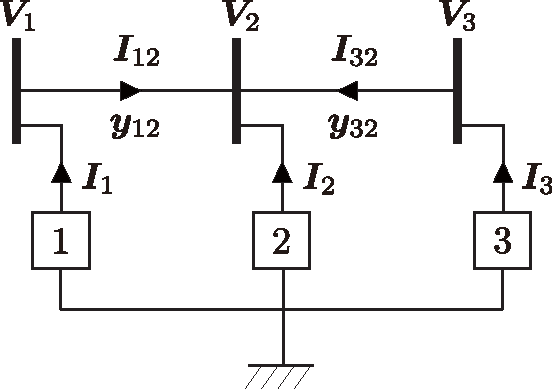
\includegraphics[width = .30\linewidth]{figs/3busex}
\caption{3つの発電機からなる電力系統モデル\red{(要変更)}}
\label{fig:3genex}
\end{figure}

\begin{figure}[t]
  \centering
  {
  \begin{minipage}{0.32\linewidth}
    \centering
    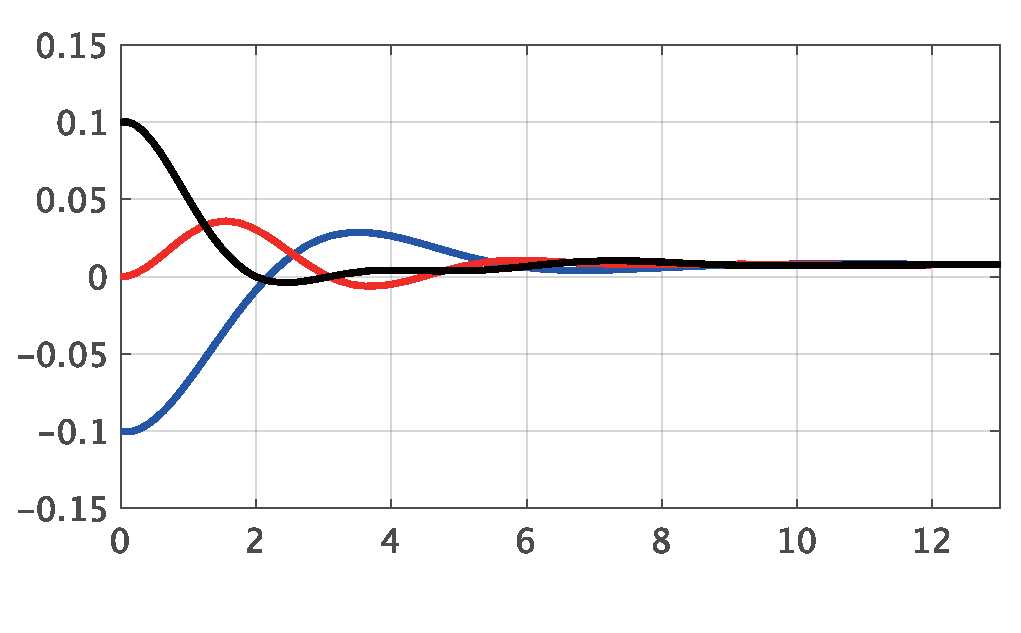
\includegraphics[width = .99\linewidth]{figs/delta}
    \subcaption{ $\delta^{\rm lin}$ }
  \end{minipage}
  \begin{minipage}{0.32\linewidth}
    \centering
    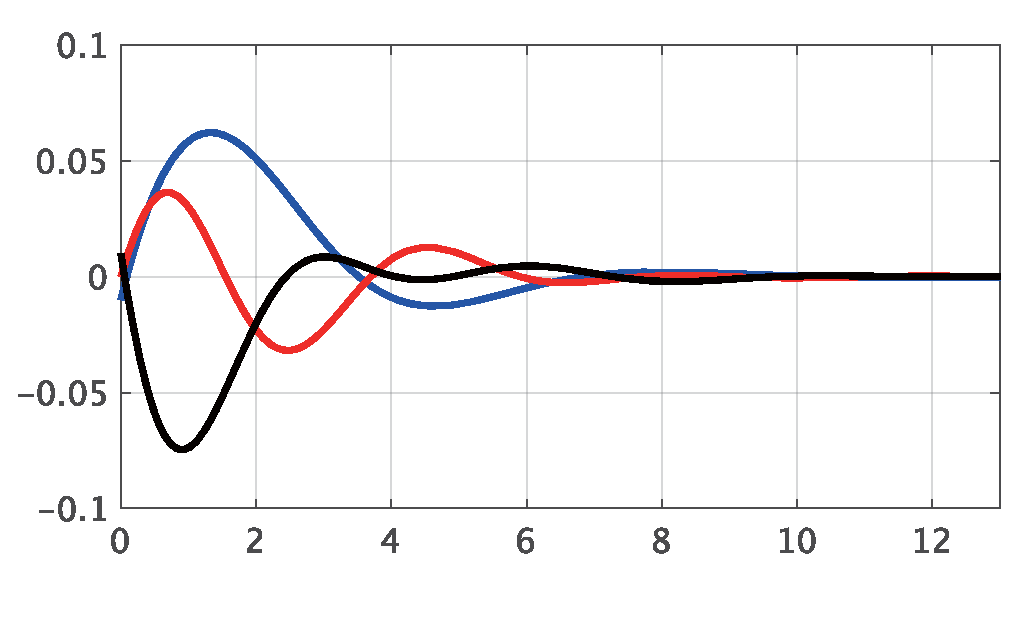
\includegraphics[width = .99\linewidth]{figs/omega}
    \subcaption{ $\Delta \omega^{\rm lin}$ }
  \end{minipage}
  \begin{minipage}{0.32\linewidth}
    \centering
    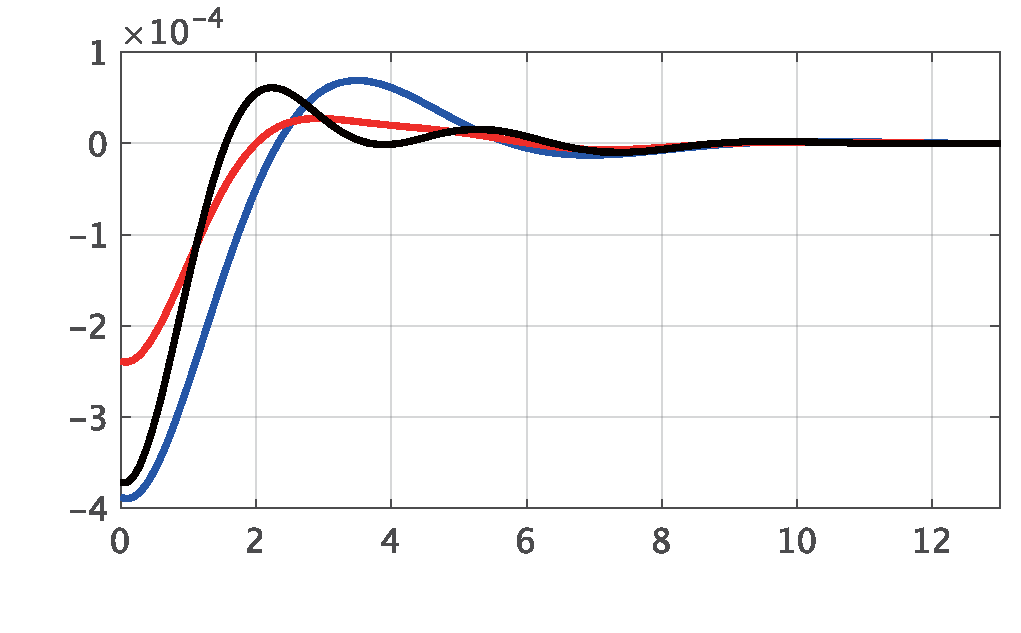
\includegraphics[width = .99\linewidth]{figs/E}
    \subcaption{ $E^{\rm lin}$ }
  \end{minipage}
  }
  \caption{近似線形モデルの初期値応答(青:発電機1,赤:発電機2,黒:発電機3)}
  \label{fig:timeex}
\end{figure}

%\begin{figure}[t!]
%\centering
%{    
%    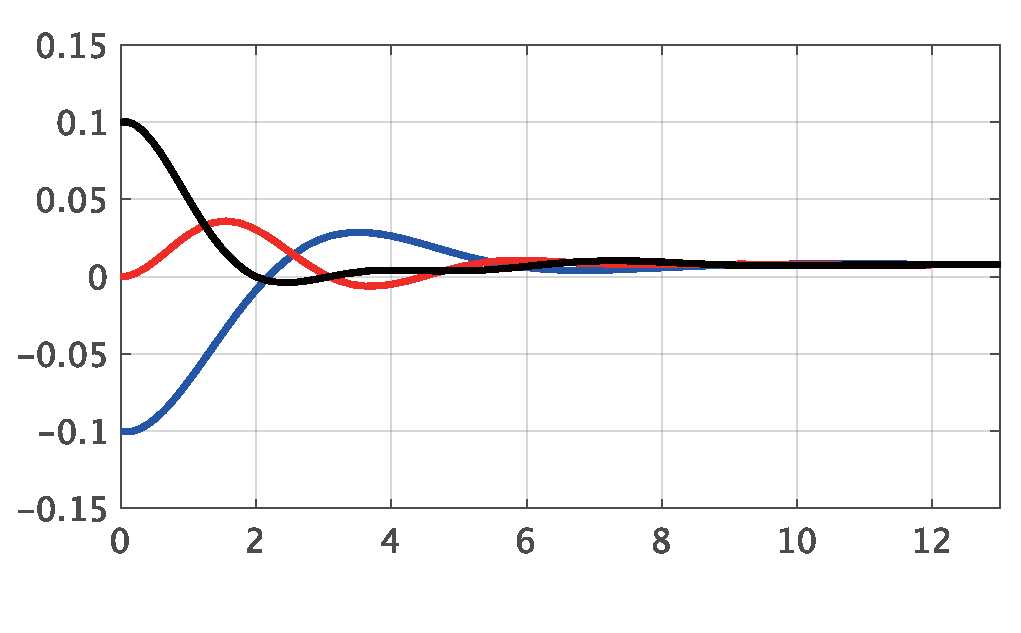
\includegraphics[width = .5\linewidth]{figs/delta}
%    \subcaption{ $\delta^{\rm lin}$ }
%    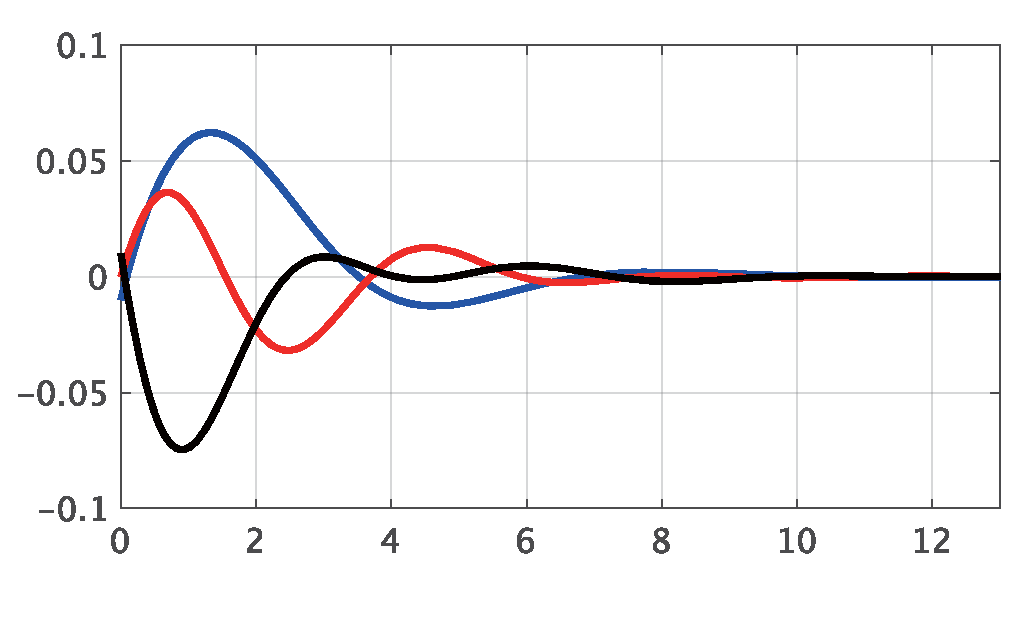
\includegraphics[width = .5\linewidth]{figs/omega}
%    \subcaption{ $\Delta \omega^{\rm lin}$ }
%    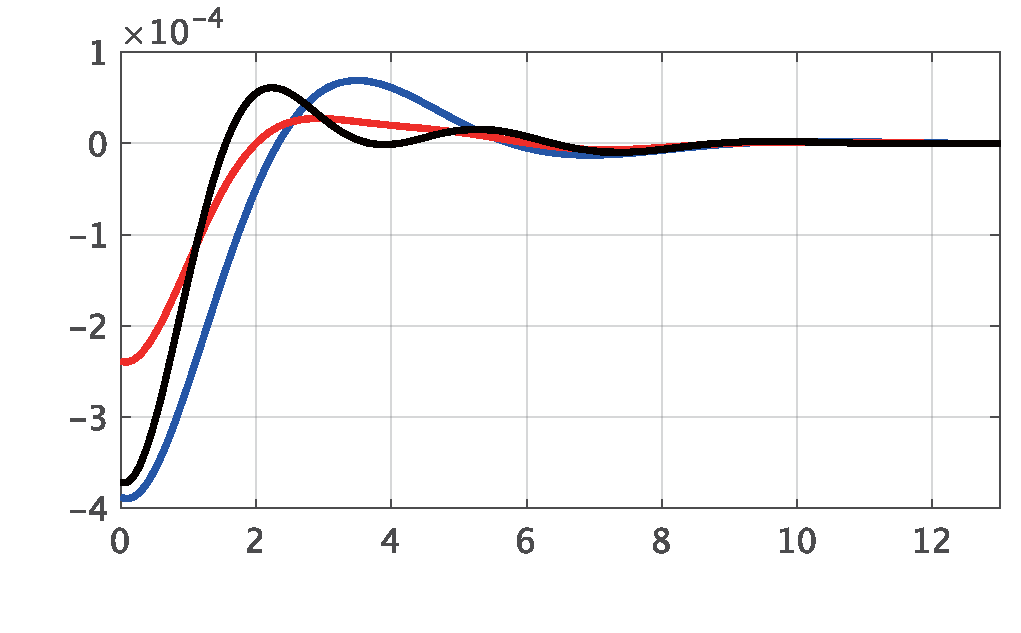
\includegraphics[width = .5\linewidth]{figs/E}
%    \subcaption{ $E^{\rm lin}$ }
%}
%\caption{近似線形モデルの初期値応答(青:発電機1,赤:発電機2,黒:発電機3)}
%\label{fig:timeex}
%\end{figure}

\begin{figure}[t]
  \centering
  {
  \begin{minipage}{0.32\linewidth}
    \centering
    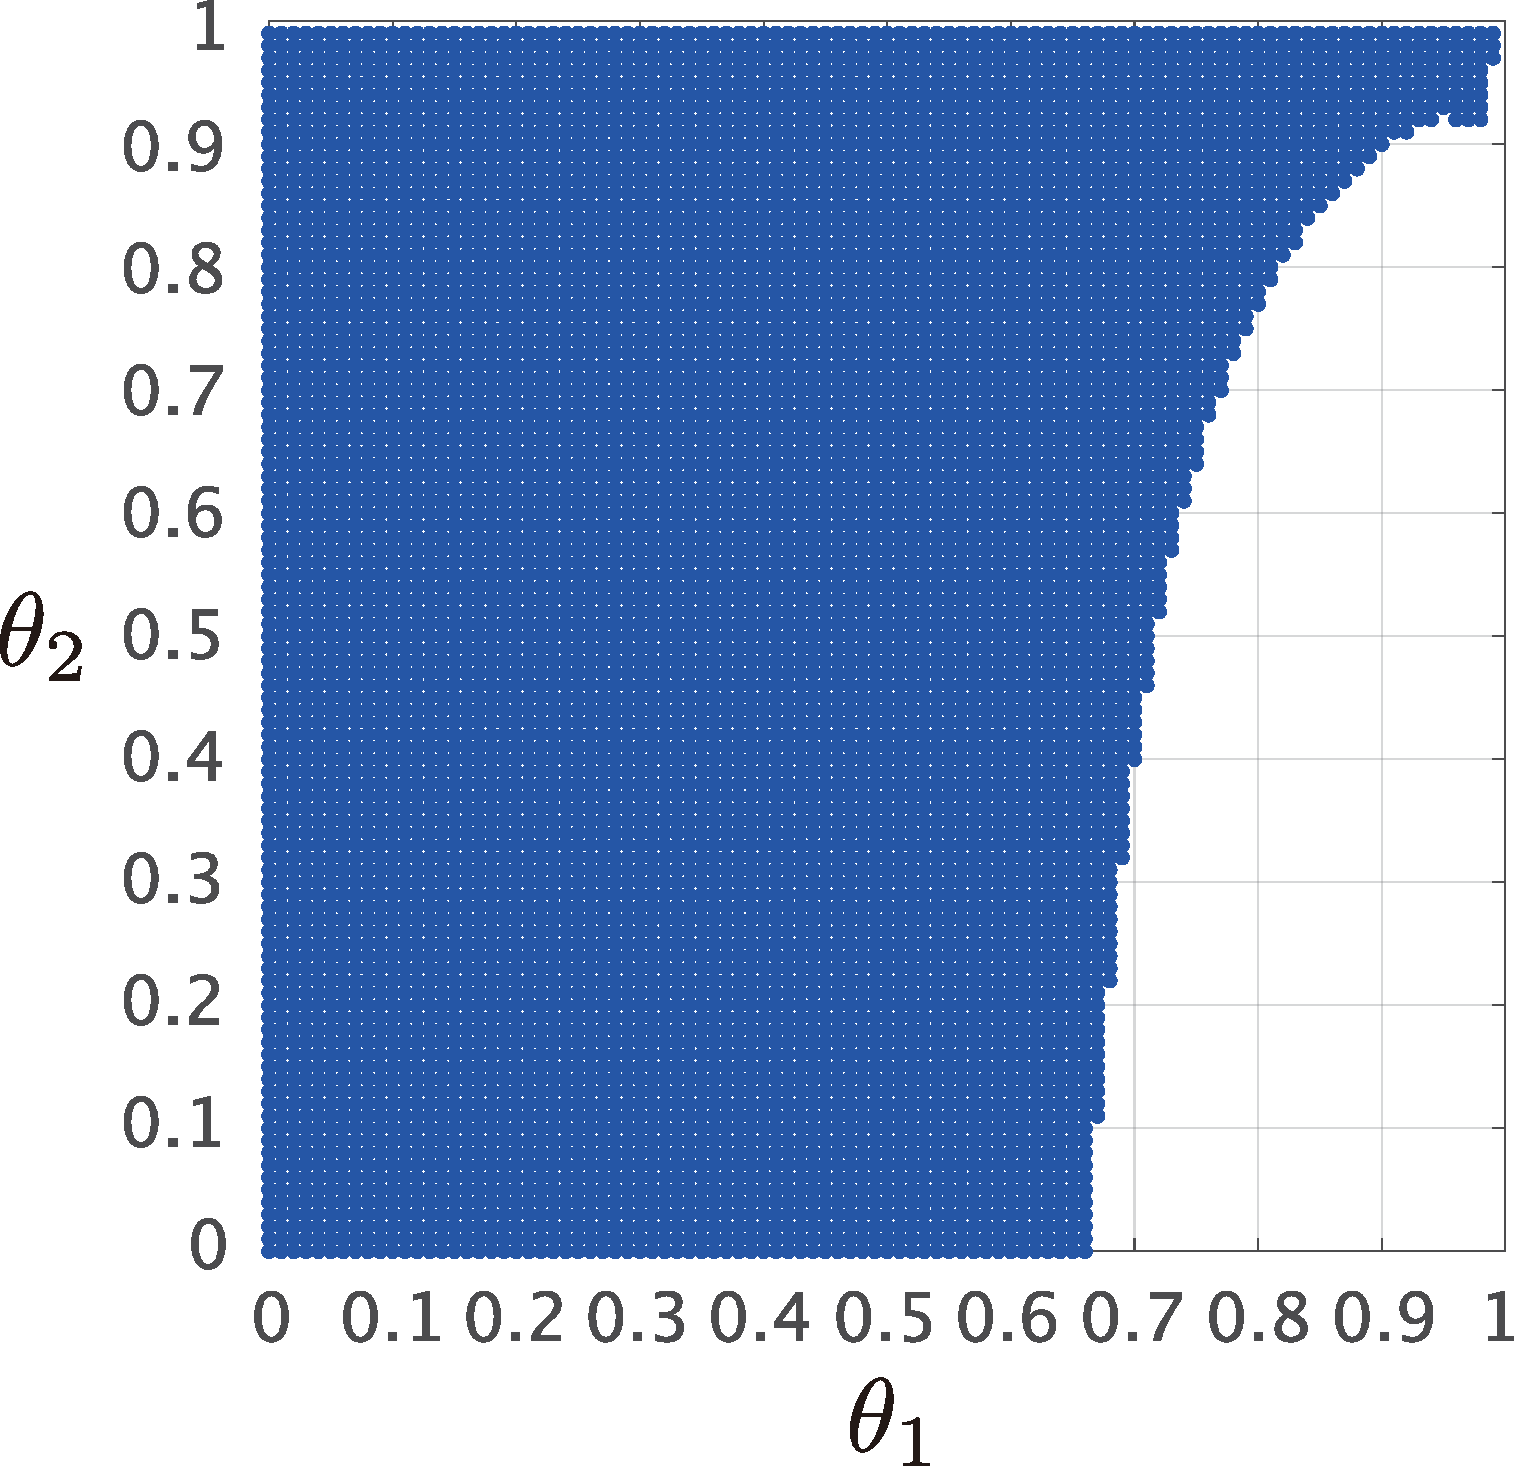
\includegraphics[width = .85\linewidth]{figs/gam01}
    \subcaption{ $\gamma=0.1$ }
  \end{minipage}
  \begin{minipage}{0.32\linewidth}
    \centering
    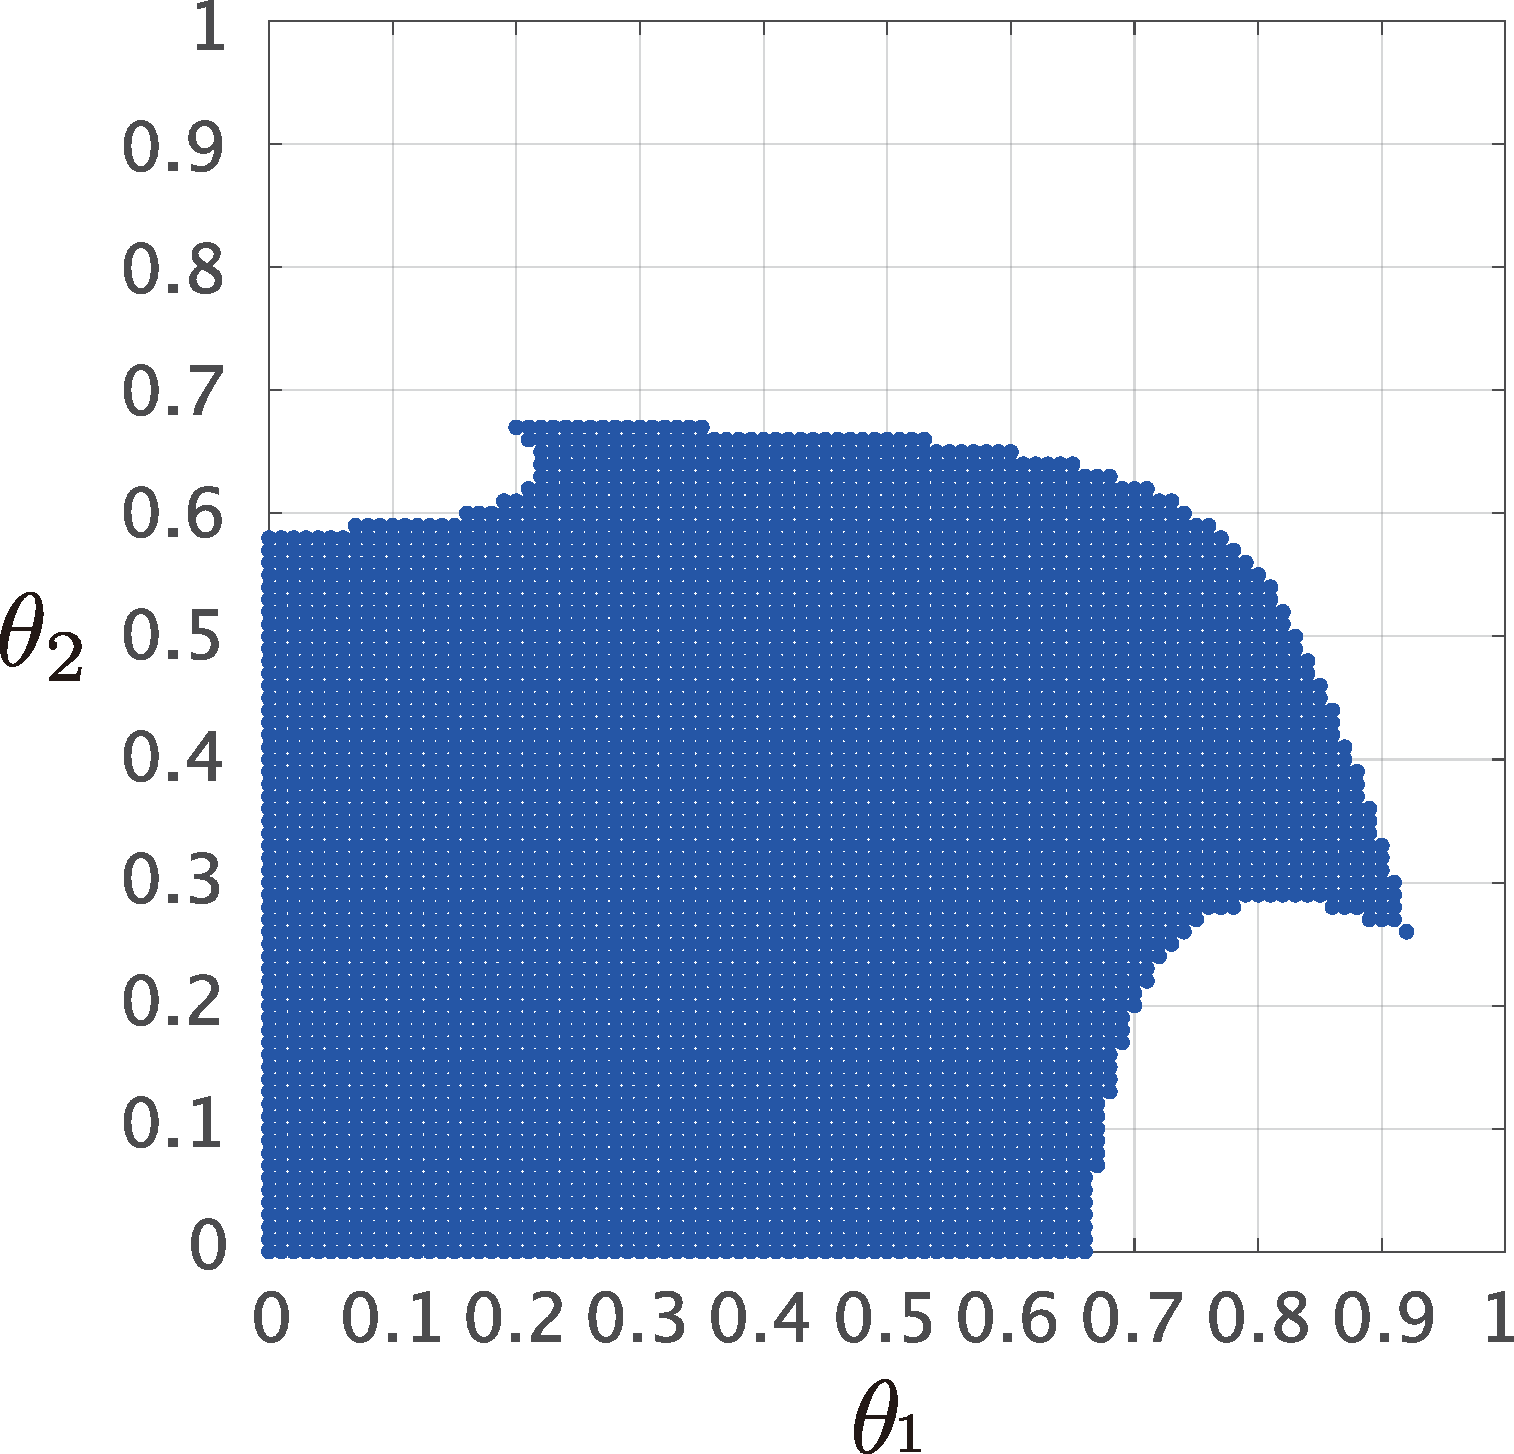
\includegraphics[width = .85\linewidth]{figs/gam2}
    \subcaption{ $\gamma=2$ }
  \end{minipage}
  \begin{minipage}{0.32\linewidth}
    \centering
    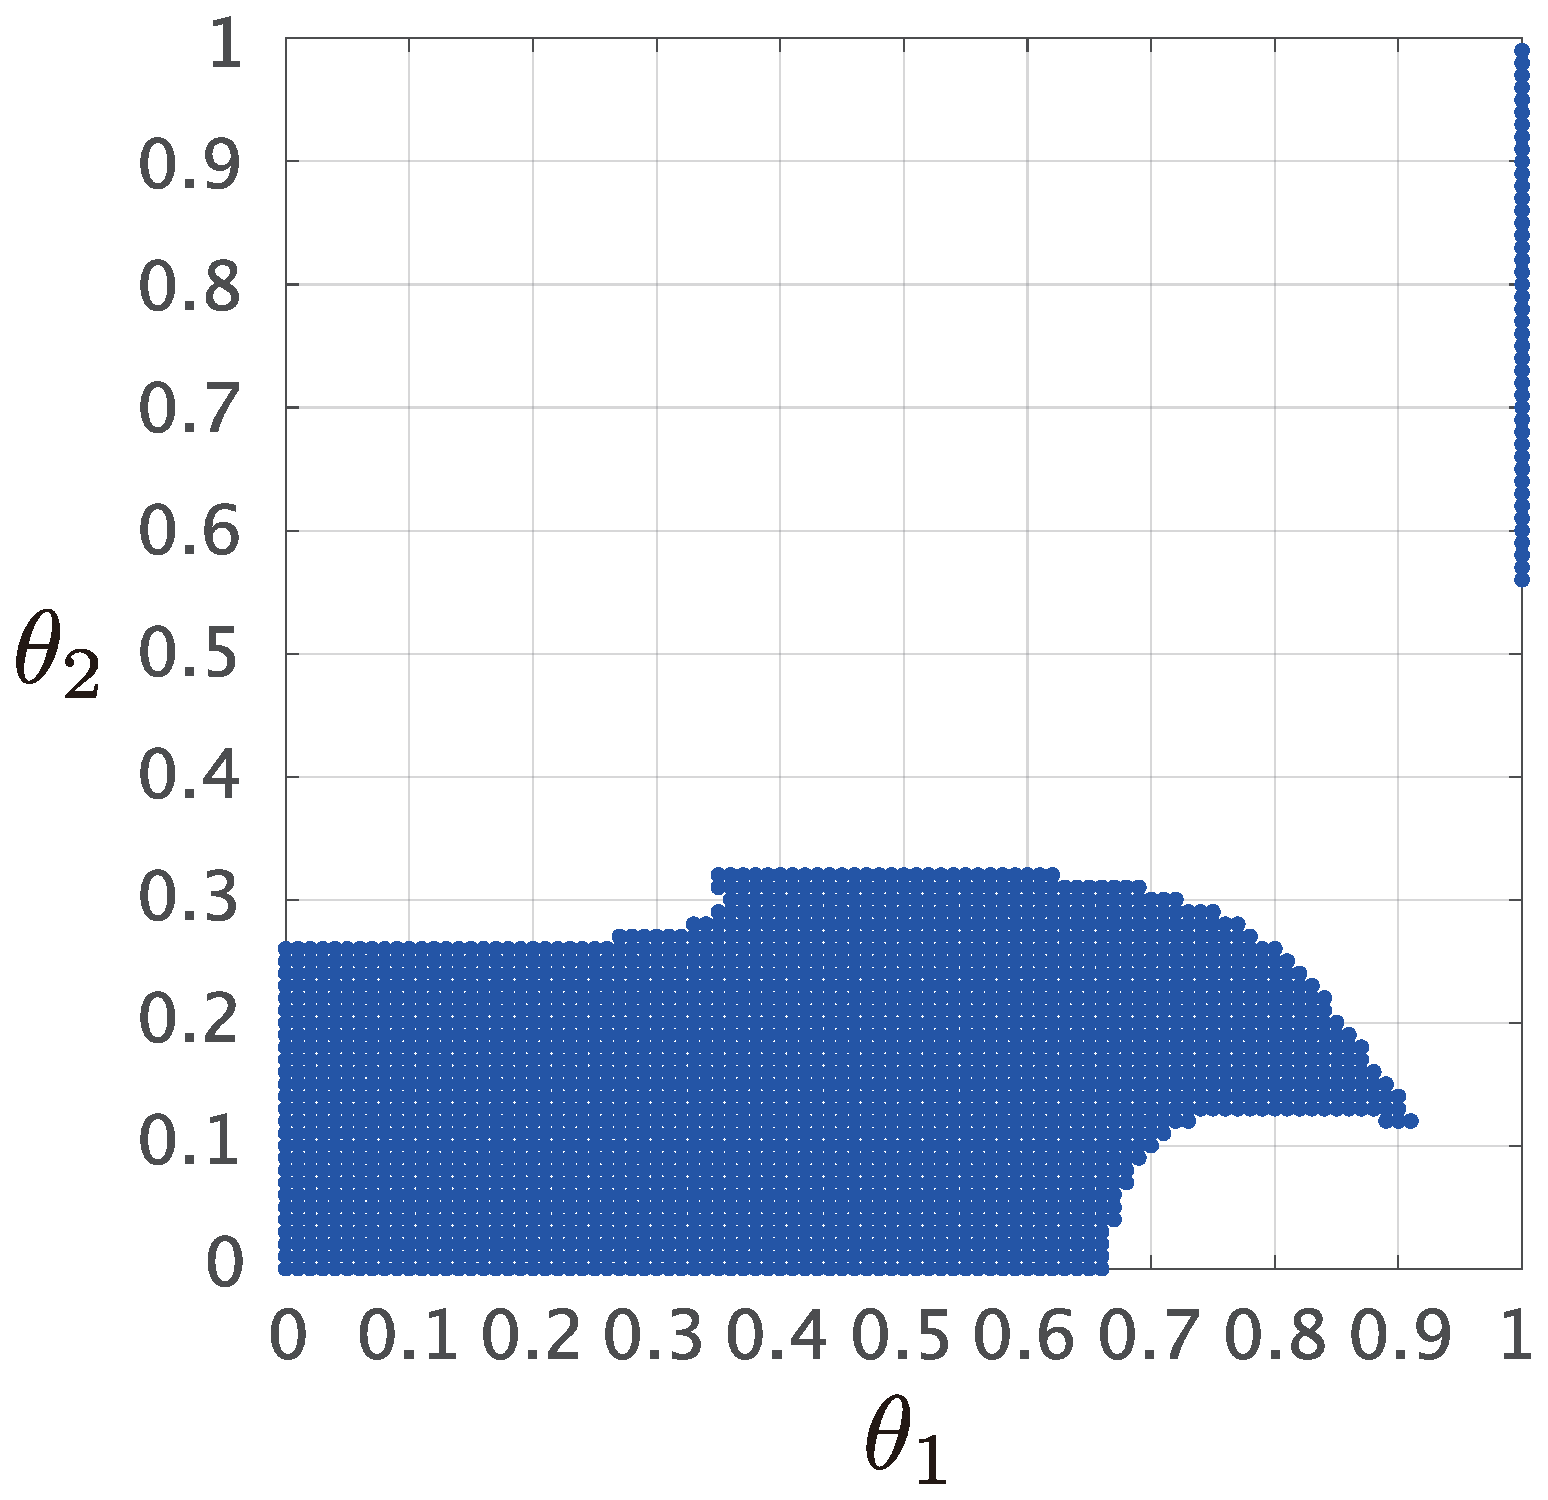
\includegraphics[width = .85\linewidth]{figs/gam5}
    \subcaption{ $\gamma=5$ }
  \end{minipage}
  \caption{近似線形モデルが安定となるパラメータの領域}
  \label{fig:gamsta}
  }
\end{figure}

\begin{例}[近似線形モデルの数値的な安定性解析]\label{ex:linsyssim}
\ref{fig:3genex}に示される3つの発電機で構成される電力系統モデルを考える。
以下では,発電機の物理定数は共通であるものとして,すべての$i \in \{1,2,3\}$に対して
\begin{align*}
M_i=1
,\qquad
D_i=1
,\qquad
\tau_{{\rm d}i} = 0.01
,\qquad
X_{{\rm d}i} = 1.01
,\qquad
X_{{\rm q}i} = 1
\end{align*}
に設定する。
また,系統周波数は$\omega_0=1$とする。

式\ref{eq:lindynu0}の近似線形モデルを導出するため,内部状態の定常値
$(\delta^{\star},E^{\star})$を設定する。
内部電圧の定常値は各発電機で異なる値として
\begin{subequations}\label{eq:exEsds}
\begin{align}
E^{\star}_1=1
,\qquad
E^{\star}_2=2
,\qquad
E^{\star}_3=3
\end{align}
に設定する。
回転子偏角差の定常値は,パラメータ$\theta_1 \in [0, 1]$を用いて
\begin{align}
\delta_{12}^{\star}= - \frac{\pi}{2} \theta_1
,\qquad
\delta_{13}^{\star}=  \frac{\pi}{2} \theta_1
\end{align}
と表す。
\end{subequations}
パラメータ$\theta_1$の大きさは,定常状態における回転子偏角差の大きさに対応している。
このパラメータの変化は,式\ref{eq:sysmats}のシステム行列の変化として近似線形モデルに現れる。
送電網のアドミタンス行列も同様に,2つのパラメータ$\gamma >0$と$\theta_2 \in [0,1]$を用いて
\begin{align*}
\bm{Y} =
\theta_2
\mat{
\gamma & 0 & 0 \\
0 &\gamma & 0 \\
0 & 0 & \gamma
}
 +
\bm{j} (1-\theta_2) 
\mat{
-1 & 1 & 0 \\
1 & -2 & 1 \\
0 & 1 & -1 
}
\end{align*}
と表す。
ここで,$\gamma$はアドミタンス行列の実部の絶対値を指定するパラメータであり,$\theta_2$は実部と虚部の相対的な大小関係を指定するパラメータである。
アドミタンス行列のパラメータ変化は,式\ref{eq:defkh}の縮約コンダクタンス$B^{\rm red}_{ij}$と縮約サセプタンス$G^{\rm red}_{ij}$の値の変化として近似線形モデルに現れる。
上記のパラメータ$(\gamma,\theta_1,\theta_2)$を変化させて,近似線形モデルの安定性を数値的に解析する。

まず,$\gamma=2$,$\theta_1=0.3$,$\theta_2=0.2$とした場合のシステムの初期値応答を確認してみよう。
適当な初期値を設定した場合の結果を\ref{fig:timeex}に示す。
この図から,このパラメータ設定の場合には,式\ref{eq:linmconv}のように発電機群の内部状態が漸近収束していることがわかる。

つぎに,(a) $\gamma=0.1$,(b) $\gamma=2$,(c) $\gamma=5$に設定する。
この(a)--(c)の場合において,$\theta_1$と$\theta_2$を0.01の刻み幅で変化させて式\ref{eq:lindynu0}の$\Psi$の固有値を調べることにより,近似線形モデルが安定であるか否かを網羅的に確認してみよう。
\ref{fig:gamsta}にその結果を示す。
近似線形モデルが安定となったパラメータを青の領域で表している。
\ref{fig:gamsta}(a)--(c)から,$\gamma$が大きくなる,すなわち,アドミタンス行列の実部であるコンダクタンス行列の絶対値が大きくなるにしたがって,近似線形モデルが安定となるパラメータの領域が狭くなっていることがわかる。

また,どの図においても原点付近のパラメータ領域,すなわち,定常状態における回転子偏角差が小さく,かつ,アドミタンス行列の実部が虚部よりも相対的に小さい場合には,近似線形モデルが安定であることがわかる。
なお,$\gamma=5$,$\theta_1=1$,$\theta_2 \in [0.56,0.99]$のパラメータでは,挙動は非常に振動的であるが,例外的に安定であった。
これらの結果から,定常状態における回転子偏角差が小さく,コンダクタンス行列がサセプタンス行列よりも相対的に小さい場合に,近似線形モデルが安定になりやすい傾向にあることがわかる。
\end{例}




\section{近似線形モデルの数学的な安定性解析\advanced}\label{sec:linmathana}

\subsection{近似線形モデルの定態安定性\advanced}

本節では,式\ref{eq:lindynu0}の近似線形モデルの安定性を数学的に解析する。
その安定性は行列$\Psi$の固有値により特徴づけられる。
一方で,第\ref{sec:numlinsta}節で議論されているように,$\Psi$は正則ではなく,その零固有値に対する固有空間は
\begin{align}\label{eq:eqset}
\mathcal{M} =
 \sfspan\left\{
 \mat{
 \mathds{1}\\
 0\\
 0
 }
 \right\}
\end{align}
である。
この固有空間は,相対的な値を一定に保ってすべての発電機の偏角を変化させた等価な定常値の集合を表している。
したがって,近似線形モデルの状態が式\ref{eq:eqset}の平衡点集合のうちのどの点に収束するかは問題とならない。
この事実に基づき,つぎの定義を与える。

\begin{定義}[近似線形モデルの定態安定性]
\label{def:stalin}
式\ref{eq:lindynu0}の近似線形モデルを考える。
任意の初期値に対して,内部状態が式\ref{eq:eqset}の平衡点集合$\mathcal{M}$のいずれかの点に収束するとき,近似線形モデルは\emph{定態安定}であると呼ぶ。
\end{定義}

定義\ref{def:stalin}における定態安定性は,任意の初期値に対して,式\ref{eq:linmconv}が成り立つことを表している。
なお,式\ref{eq:linmconv}において$c_0$の値は任意であるため,その任意性を「$\mathcal{M}$のいずれかの点に収束すること」として表現している。

以下の議論では,式\ref{eq:lindynu0}の$\Psi$の核空間は1次元であり,$\sfker \Psi = \mathcal{M}$が成り立つことを仮定する。
これは近似線形モデルが定態安定であるための必要条件である。
特に,$A$が正則である場合には,
\begin{align}\label{eq:defL0}
L_0:= L-CA^{-1}B 
\end{align}
を用いて,その必要条件は
\begin{align}\label{eq:nescon}
\sfker L_0 = \sfspan
\left\{
\mathds{1}
\right\}
\end{align}
と表せる。
なお,この行列$L_0$は,のちの解析で重要な役割を果たす。
以下の議論のため,つぎの基本的な用語を導入する。

\begin{定義}[正方行列の安定性]
\label{def:matsta}
正方行列$A$に対して,そのすべての固有値の実部が負であるとき,$A$は\emph{安定}であると呼ぶ。
\end{定義}



\subsection{近似線形モデルの受動性\advanced}\label{sec:linpasana}

\subsubsection{近似線形モデルのフィードバック系による表現}

式\ref{eq:lindynu0}の近似線形モデルを2つのサブシステムのフィードバック系として記述することを考える。
1つ目のサブシステムは,周波数偏差に関する微分方程式系として
\begin{align}\label{eq:Fss}
F: \simode{
M \Delta \dot{\omega}^{\rm lin} &= -D \Delta \omega^{\rm lin}
+
u_F \\
y_F &= \omega_0 \Delta \omega^{\rm lin}
}
\end{align}
とする。
以下では,このサブシステムを\emph{機械サブシステム}と呼ぶ。
機械サブシステムは,発電機群の物理定数である$(M_i,D_i)_{i\in \mathcal{I}_{\rm G}}$や基準周波数$\omega_0$のみで定まり,内部状態の定常値$(\delta^{\star},E^{\star})$には依存しない。

2つ目のサブシステムは,回転子偏角と内部電圧に関する微分方程式系として
\begin{align}\label{eq:Gss}
G: \simode{
\dot{\delta}^{\rm lin} & = u_G \\
\tau_{\rm d} \dot{E}^{\rm lin} &= A E^{\rm lin} + B \delta^{\rm lin} \\
y_G &= C E^{\rm lin} + L \delta^{\rm lin}
}
\end{align}
とする。
このサブシステムを\emph{電気サブシステム}と呼ぶ。
電気サブシステムは,発電機群の物理定数である$(\tau_{{\rm d}i})_{i\in \mathcal{I}_{\rm G}}$
だけでなく,内部状態の定常値$(\delta^{\star},E^{\star})$にも依存する。
実際,式\ref{eq:sysmats}のシステム行列$(L,A,B,C)$は,$(\delta^{\star},E^{\star})$の関数である。
これら2つのサブシステムの入出力を
\begin{align}\label{eq:nfedcon}
u_F = -y_G,\qquad
u_G = y_F
\end{align}
のようにネガティブ・フィードバック結合すれば,式\ref{eq:lindynu0}の近似線形モデルが表現される。
以降の定態安定性の解析は,機械サブシステムと電気サブシステムの受動性と呼ばれる性質に基づく。
受動的なサブシステムのネガティブ・フィードバック系は安定であることが知られている。


\subsubsection{機械サブシステムの受動性}

式\ref{eq:Fss}の機械サブシステム$F$は,つぎで定義される強受動性をもつ。

\begin{定義}[線形システムの受動性]\label{def:passivelin}
線形システム
\begin{align}\label{eq:siglin}
\Sigma: \simode{
\dot{x} &= Ax + Bu \\
y &= Cx 
}
\end{align}
を考える。
対称行列$P$を用いて,関数
\begin{align}\label{eq:defstlin}
W(x):= \frac{1}{2}x^{\sf T}Px
\end{align}
を定義する。
任意の$u$に対して
\begin{align}\label{eq:conpvlin}
\frac{d}{dt} W\bigl( x(t) \bigr) \leq u^{\sf T}(t) y(t)
,\qquad
t \geq 0
\end{align}
を満たす半正定行列$P$が存在するとき,$\Sigma$は\emph{受動的}であると呼ぶ。
特に,上記の半正定行列に加えて
\begin{align}\label{eq:conosplin}
\frac{d}{dt} W\bigl( x(t) \bigr) \leq u^{\sf T}(t) y(t) -\rho \left\|y(t) \right\|^2
,\qquad
t \geq 0
\end{align}
を満たすある定数$\rho >0$が存在するとき,$\Sigma$は\emph{強受動的}であると呼ぶ
\footnote{
式\ref{eq:conosplin}の不等式は,関数$W$の表されるある種のエネルギーが,式\ref{eq:conpvlin}と比較して,出力の2乗に比例する項だけ多く消散するような受動性となっている。
このような受動性は,精確には\emph{出力強受動性}と呼ばれる。
また,$W$は\emph{蓄積関数}と呼ばれる。
}。
\end{定義}

式\ref{eq:Fss}の機械サブシステム$F$が強受動性をもつことは,以下のように確かめられる。
まず,サブシステムを
\begin{align}
F: \simode{
\dot{x}_F & = A_F x_F + B_F u_F \\
y_F &= C_F x_F
}
\end{align}
の形式で書き表す。
ただし,状態$x_F$は$\Delta \omega^{\rm lin}$を表し,システム行列は
\[
A_F := -M^{-1}D,\qquad
B_F := M^{-1},\qquad
C_F := \omega_0 I
\]
である。
また,対称行列$P_F$を
\[
P_F := \omega_0 M
\]
と定義する。
この$P_F$は正定である。
このとき,
\[
A^{\sf T}_F P_F + P_F A_F \preceq  
- \frac{ 2 \sfmin \left\{ D_i \right\}}{\omega_0} C_F^{\sf T} C_F
,\qquad
P_F B_F = C_F^{\sf T}
\]
が成り立つ。
したがって,関数$W_F(x_F):= \frac{1}{2}x_F^{\sf T}P_Fx_F$の時間微分は
\begin{align}\label{eq:Flyapeq}
\spliteq{
\frac{d}{dt} W_F \bigl( x_F (t) \bigr)
& = 
\frac{\partial W_F}{\partial x_F} \frac{d x_F}{dt} 
 \\
&=  x_F^{\sf T}(t) P_F \dot{x}_F(t) \\
 & = y_F^{\sf T}(t) u_F(t)
 + \frac{1}{2} x_F^{\sf T}(t) \left(A^{\sf T}_F P_F + P_F A_F\right) x_F(t) \\
& \leq 
y_F^{\sf T}(t) u_F(t)
- \frac{\sfmin \left\{ D_i \right\}}{\omega_0}
\|y_F(t) \|^2
}
\end{align}
と評価できる。
このことから,式\ref{eq:Fss}の機械サブシステム$F$は,任意の正定数$(M_i,D_i)_{i \in \mathcal{I}_{\rm G}}$に対して強受動的であることがわかる。


\subsubsection{電気サブシステムの受動性}


つぎに,式\ref{eq:Gss}の電気サブシステム$G$を考える。
機械サブシステム$F$とは異なり,電気サブシステム$G$は,限られた条件のもとでしか受動性をもたない。
天下り的であるが,式\ref{eq:figi}における縮約コンダクタンスがすべて0である場合,すなわち,
\begin{align}\label{eq:Gredcon}
G^{\rm red}_{ij}=0,\qquad 
\forall (i, j) \in \mathcal{I}_{\rm G} \times \mathcal{I}_{\rm G}
\end{align}
である場合を考える。
特別な場合を除いて,式\ref{eq:Gredcon}の条件は,電力系統におけるすべての送電線のコンダクタンスが0である場合にのみ成り立つ。
このとき,式\ref{eq:defkh}の関数$k_{ij}(\delta_{ij})$,$h_{ij}(\delta_{ij})$に対して,
\begin{align*}
k_{ij}(\delta_{ij}^{\star}) =
k_{ji}(\delta_{ji}^{\star})
,\qquad
h_{ij}(\delta_{ij}^{\star}) = 
- h_{ji}(\delta_{ji}^{\star}),\qquad
h_{ii}(\delta_{ii}^{\star}) = 0
\end{align*}
が成り立つ。
したがって,式\ref{eq:sysmats}のシステム行列$(L,A,B,C)$について,
\begin{align}\label{eq:sysmatst}
L=L^{\sf T} ,\qquad
\hat{A} = \hat{A}^{\sf T},\qquad
C= -\hat{B}^{\sf T}
\end{align}
が成り立つ。
以下では,この特別なシステム行列の対称構造を用いて,電気サブシステムの受動性を解析する。

まず,式\ref{eq:Gss}の電気サブシステム$G$を
\begin{align}
G: \simode{
\dot{x}_G & = A_G x_G + B_G u_G \\
y_G &= C_G x_G
}
\end{align}
の形式で表現する。
ただし,状態$x_G$は${\delta}^{\rm lin}$と$ E^{\rm lin} $を並べたベクトルであり,対称行列
\begin{align}\label{eq:hatA0}
\check{A}:= 
\hat{A}- \sfdiag \left(
\frac{X_{{\rm d}i}}{X_{{\rm q}i}(X_{{\rm d}i}-X_{{\rm q}i})}
\right)_{i \in \mathcal{I}_{\rm G} }
\end{align}
および,正定な対角行列
\[
 \Omega :=
\sfdiag \left( \sqrt{\frac{X_{{\rm d}i} -  X_{{\rm q}i}}{\tau_{{\rm d}i}} } \right)_{i \in \mathcal{I}_{\rm G} }
\]
を用いて,システム行列を
\[
A_G := 
\mat{
0 & 0 \\
 \Omega^2 \hat{B}   &  \Omega^2 \check{A} 
},\qquad
B_G := 
\mat{
I \\
0
},\qquad
C_G := 
\mat{
L & -\hat{B}^{\sf T}
}
\]
と表す。
また,対称行列$P_G$を
\begin{align}\label{eq:defPG}
P_G := 
\mat{
L  &  - \hat{B}^{\sf T} \\
- \hat{B} & -\check{A}
}
\end{align}
と定義する。
このとき,
\begin{align}\label{eq:lyapinG}
A^{\sf T}_G P_G + P_G A_G \preceq 
0
,\qquad
P_G B_G = C_G^{\sf T}
\end{align}
が成り立つ。
なお,左の行列不等式が成り立つことは,以下のように確かめられる。
不等式の左辺を計算すると,対称行列$\check{A}_{\Omega} := \Omega \check{A} \Omega$を用いて
\[
A^{\sf T}_G P_G + P_G A_G
=
\mat{
\Omega \hat{B} \\
\Omega^{-1}
}^{\sf T}
\underbrace{
\mat{
-I & -\check{A}_{\Omega} \\
-\check{A}_{\Omega} & - \check{A}_{\Omega}^2
}
}_{Y}
\mat{
\Omega \hat{B} \\
\Omega^{-1}
}
\]
と表せることがわかる。
ここで,$Y$の左上ブロック$- I$が負定であり,かつ,$Y$の$-I$に関するシューア補行列は0であることから,$Y$は半負定である。
これは,式\ref{eq:lyapinG}の行列不等式が成り立つことを意味する。


式\ref{eq:lyapinG}の関係を用いることにより,関数$W_G(x_G):= \frac{1}{2}x_G^{\sf T}P_Gx_G$の時間微分は,式\ref{eq:Flyapeq}と同様にして
\begin{align}\label{eq:Glyapeq}
\frac{d}{dt} W_G \bigl( x_G (t) \bigr)
 \leq 
y_G^{\sf T}(t) u_G(t)
\end{align}
と評価できる。
ただし,$G$の受動性を示すためには,式\ref{eq:defPG}の$P_G$は半正定でなければならない。
ここで,式\ref{eq:sysmats}の行列$A$が安定である場合には,
\[
A= S^2 \check{A}
\qquad \Longleftrightarrow \qquad S^{-1} A S = S \check{A} S
\]
であることから,$S \check{A} S$の固有値はすべて負であることが導かれる。
ただし,
\[
S:=\sfdiag \left( \sqrt{X_{{\rm d}i} -  X_{{\rm q}i} }\right)_{i \in \mathcal{I}_{\rm G} } 
\]
である。
これは,$ \check{A} $が負定であることを意味する。
このとき,式\ref{eq:defPG}の$P_G$が半正定であるための必要十分条件は,$ -\check{A} $に関するシューア補行列が半正定であること,すなわち,
\begin{align}\label{eq:pdsp}
L_0 =L_0^{\sf T} \succeq 0
\end{align}
が成り立つことである。
ただし,式\ref{eq:defL0}の$L_0$に対して,式\ref{eq:sysmatst}から
\[
L_0 = L + \hat{B}^{\sf T} \check{A}^{-1} \hat{B}
\]
であることを用いた。

以上より,式\ref{eq:sysmats}のシステム行列$(L,A,B,C)$について
\begin{itemize}
\item[(i)] 行列$A$が安定である
\item[(ii)] 式\ref{eq:Gredcon}のように縮約コンダクタンスがすべて0である
\item[(iii)] 式\ref{eq:defL0}の行列$L_0$に対して,式\ref{eq:pdsp}の行列不等式が成り立つ
\end{itemize}
という3つの条件が満たされる場合には,式\ref{eq:Gss}の電気サブシステム$G$は受動的であることがわかる。
以下では,上記の条件(i)--(iii)をまとめて,\emph{受動送電条件}と呼ぶ。
なお,個別には受動送電条件(i)などと呼ぶ。

これまでの議論より,受動送電条件が電気サブシステム$G$が受動的であるための十分条件であることが示された。
一方で,この条件は,電気サブシステムの受動性や任意の物理定数に対する近似線形モデルの定態安定性のための必要条件であることも示される。
詳細は,第\ref{sec:nesconana}節と第\ref{sec:nesconsta}節で後述する。

\subsection{受動性に基づく定態安定性の解析\advanced}

\subsubsection{フィードバック系の安定性解析}

以下では,受動送電条件のもと,電気サブシステムが受動的である場合に,それらのフィードバック系の安定性,すなわち,式\ref{eq:lindynu0}の近似線形モデルの定態安定性を解析する。
式\ref{eq:Flyapeq}と式\ref{eq:Glyapeq}の不等式が成り立つことから,それらの和は
\begin{align*}
\spliteq{
 \frac{d}{dt} \bigl\{ W_F \bigl( x_F (t) \bigr)
& +
 W_G \bigl( x_G (t) \bigr)
 \bigr\} \\
& \leq 
y_F^{\sf T}(t) u_F(t)
+
y_G^{\sf T}(t) u_G(t)
- \frac{\sfmin \left\{ D_i \right\}}{\omega_0}
\|y_F(t) \|^2
}
\end{align*}
となる。
この不等式に,式\ref{eq:nfedcon}のフィードバック結合の方程式を代入すれば,
\begin{align}\label{eq:FGlyapeq}
 \frac{d}{dt} \bigl\{ W_F \bigl( x_F (t) \bigr)
 +
 W_G \bigl( x_G (t) \bigr)
 \bigr\} 
 \leq 
- \frac{\sfmin \left\{ D_i \right\}}{\omega_0}
\|y_F(t) \|^2
\end{align}
を得る。
すなわち,関数$W_F$と$W_G$の和は,時間に関して単調非増加である。
また,$W_F$と$W_G$の下限値はどちらも0であることから,時間が十分に経過するとそれらの和はある値に漸近収束する。
これは,式\ref{eq:FGlyapeq}の左辺の時間微分が0に漸近収束することを意味する。
また,式\ref{eq:FGlyapeq}の右辺は,$y_F(t)\neq 0$であるとき負であり,$y_F(t)=0$であるときのみ0であることから,
\begin{align}\label{eq:yFlim0}
\lim_{t\rightarrow \infty} y_F(t)  =0
\end{align}
が得られる。
さらに,式\ref{eq:Fss}の出力方程式に注目すると,出力$y_F$は内部状態$\Delta \omega^{\rm lin}$の定数倍であることから,機械サブシステム$F$に対して,
\begin{align}\label{eq:Fobs}
y_F(t)  =0,\quad \forall t\geq 0 
\quad \Longrightarrow \quad
\Delta \omega^{\rm lin}(t)  =0,\quad \forall t\geq 0 
\end{align}
が成り立つことがわかる。
これは,システム制御工学において\emph{可観測性}と呼ばれる性質である
\footnote{
式\ref{eq:siglin}の線形システム$\Sigma$について,出力$y(t)$が恒等的に0であるならば,内部状態$x(t)$も恒等的に0であるとき,$\Sigma$は\emph{可観測}であると呼ばれる。
また,$\Sigma$が可観測であるための必要十分条件は
\[
\sfker \mat{
C \\
CA \\
\vdots \\
CA^{n-1}
}
=\{0\}
\]
である。
ただし,$n$は状態の次元である。
}。
したがって,式\ref{eq:yFlim0}と式\ref{eq:Fobs}から,
式\ref{eq:lindynu0}の近似線形モデルについて,
任意の初期値$(\Delta \omega^{\rm lin}(0),\delta^{\rm lin}(0),E^{\rm lin}(0))$に対して,
\begin{align}\label{eq:Delom0}
\lim_{t\rightarrow \infty} \Delta \omega^{\rm lin}(t)  =0
\end{align}
が成り立つことがわかる。
すなわち,フィードバック系における式\ref{eq:Fss}の機械サブシステム$F$の内部状態は0に漸近収束する。

一方で,式\ref{eq:Gss}の電気サブシステム$G$の内部状態が同様に0に漸近収束することは,以上の議論からは導くことはできない。
具体的には,式\ref{eq:nfedcon}の関係と式\ref{eq:Delom0}の漸近収束から,2つのサブシステムの入出力に関して
\[
\lim_{t\rightarrow \infty} u_F(t)  =0,\qquad
\lim_{t\rightarrow \infty} u_G(t)  =0,\qquad
\lim_{t\rightarrow \infty} y_G(t)  =0
\]
が導かれる。
しかしながら,電気サブシステムは可観測ではないため,その内部状態が漸近収束することまでは結論できない。
電気サブシステムが可観測であると仮定すると,任意の初期値に対して
\[
\lim_{t\rightarrow \infty}  \delta^{\rm lin}(t)  =0,\qquad
\lim_{t\rightarrow \infty}  E^{\rm lin}(t)  =0
\]
となるが,これは式\ref{eq:linmconv}において必ず$c_0=0$となることを意味する。
この事実は,式\ref{eq:lindynu0}の$\Psi$が零固有値をもつため安定でないことと矛盾する。
なお,特別な場合を除いて,電気サブシステムは可制御ではある
\footnote{
式\ref{eq:siglin}の線形システム$\Sigma$について,
各々すべての初期値$x(0)$に対して,ある時刻$T > 0$において $x(T) = 0$ となる入力$u(t)$が存在するとき,$\Sigma$は\emph{可制御}であると呼ぶ。
また,$\Sigma$が可制御であるための必要十分条件は
\[
\sfim \mat{
B & AB & \cdots &A^{n-1}B
}
= \mathbb{R}^n
\]
である。
ただし,$n$は状態の次元である。
}。


\subsubsection{不可観測な状態変数を分離する基底変換}

式\ref{eq:Gss}の電気サブシステム$G$から,不可観測な回転子偏角の共通成分を取り除くことで,可観測なサブシステムを導出することを考える。
具体的には,式\ref{eq:lindyn}の状態$\delta^{\rm lin}$に対して基底変換を適用することにより,回転子偏角の偏差のみを記述する微分方程式系を導出する。
なお,以下で説明する基底変換は,受動送電条件が成り立つか否かに関わらず常に適用可能である。

ある行列$W \in \mathbb{R}^{N\times (N-1)}$を用いて,$\delta^{\rm lin}$を
\begin{align}\label{eq:batrinv}
\delta^{\rm lin}
=
W
\delta^{\rm lin}_{\rm e} +
\mathds{1}
\overline{\delta}^{\rm lin}_{\rm e}
\end{align}
のように展開する。
ここで,$\mathds{1}$は$\delta^{\rm lin}$の共通成分を表す基底であり,$W$はそれ以外の偏差成分を表す基底である。
すなわち,$\delta^{\rm lin}$の共通成分が$\overline{\delta}^{\rm lin}_{\rm e}$であり,偏差成分が$\delta^{\rm lin}_{\rm e}$である。
なお,共通成分$\overline{\delta}^{\rm lin}_{\rm e}$は1次元であり,偏差成分$\delta^{\rm lin}_{\rm e}$は$(N-1)$次元である。

つぎに,式\ref{eq:batrinv}の逆変換を考える。
具体的には,
\[
\delta^{\rm lin}
=
\underbrace{
\mat{
W & \mathds{1}
}
}_{T}
\mat{
\delta^{\rm lin}_{\rm e} \\
\overline{\delta}^{\rm lin}_{\rm e}
}
\quad
\Longleftrightarrow
\quad
\mat{
\delta^{\rm lin}_{\rm e} \\
\overline{\delta}^{\rm lin}_{\rm e}
}
=
\underbrace{
\mat{
W^{\dagger} \\
\frac{1}{N} \mathds{1}^{\sf T}
}
}_{T^{-1}}
\delta^{\rm lin}
\]
となる行列$W^{\dagger} \in \mathbb{R}^{(N-1)\times N}$を考える。
ただし,この逆変換が存在するためには,$W$の列ベクトルは$\mathds{1}$と直交するものでなければならない。
このことはつぎのように確かめられる。
逆変換の関係から
\begin{align*}
T^{-1}T
=\mat{
W^{\dagger}W & W^{\dagger} \mathds{1}\\
\frac{1}{N} \mathds{1}^{\sf T} W & \frac{1}{N} \mathds{1}^{\sf T} \mathds{1}
}
=\mat{
I & 0\\
0 & 1
}
\end{align*}
が成り立たなければならない。
すなわち,$W$と$W^{\dagger}$は
\[
\mathds{1}^{\sf T} W=0,\qquad
W^{\dagger}W=I,\qquad
W^{\dagger} \mathds{1}=0
\]
を満たす行列である。
したがって,1つ目の等式から,$W$の列ベクトルは$\mathds{1}$と直交することがわかる。
なお,$W$と$W^{\dagger}$は,
$V \mathds{1}=0$,
$\mathds{1}^{\sf T} U=0$
を満たし,かつ,$VU$が正則となる適当な行列$V \in \mathbb{R}^{(N-1) \times N}$と$U\in \mathbb{R}^{N\times (N-1)}$を用いて
\[
W = U(VU)^{-1},\qquad
W^{\dagger}=V
\]
とすれば構成できる。
このとき,2つの積$WW^{\dagger}$は$\sfspan\{\mathds{1}\}$の直交補空間への直交射影行列となり
\begin{align}\label{eq:psudinv}
WW^{\dagger} = I - \frac{1}{N} \mathds{1} \mathds{1}^{\sf T}
\end{align}
と表せる。
このような$W$の擬似逆行列$W^{\dagger}$は,特別に\emph{ムーア・ペンローズの擬似逆行列}と呼ばれる。


式\ref{eq:Gss}の電気サブシステム$G$に上述の基底変換を適用する。
まず,$\delta^{\rm lin}$に関する微分方程式に式\ref{eq:batrinv}を代入すると
\[
W
\dot{\delta}^{\rm lin}_{\rm e} +
\mathds{1}
\dot{\overline{\delta}}^{\rm lin}_{\rm e}=u_G
\]
が得られる。
この微分方程式に左から$W^{\dagger}$または$\frac{1}{N} \mathds{1}^{\sf T}$を乗じれば
\[
\dot{\delta}^{\rm lin}_{\rm e} = W^{\dagger} u_G,\qquad
\dot{\overline{\delta}}^{\rm lin}_{\rm e} = \frac{1}{N} \mathds{1}^{\sf T} u_G
\]
を得る。
つぎに,行列$L$と$B$に式\ref{eq:LBker}の関係が成り立つことに注意すると,$E^{\rm lin}$に関する微分方程式と出力方程式は
\[
\tau_{\rm d} \dot{E}^{\rm lin} = A E^{\rm lin} + 
B W {\delta}^{\rm lin}_{\rm e}
, \qquad
y_G = C E^{\rm lin} + 
L W {\delta}^{\rm lin}_{\rm e}
\]
と書き換えられる。
したがって,基底変換された電気サブシステムが
\begin{align}\label{eq:Gsstr}
G: \simode{
\dot{\overline{\delta}}^{\rm lin}_{\rm e} & = \frac{1}{N} \mathds{1}^{\sf T} u_G \\
\dot{\delta}^{\rm lin}_{\rm e} & = W^{\dagger}u_G \\
\tau_{\rm d} \dot{E}^{\rm lin} &= A E^{\rm lin} + B W {\delta}^{\rm lin}_{\rm e} \\
y_G &= C E^{\rm lin} + L W {\delta}^{\rm lin}_{\rm e}
}
\end{align}
と得られる。
このシステム表現で注目すべき点は,$\delta^{\rm lin}$の共通成分を表す${\overline{\delta}}^{\rm lin}_{\rm e}$は,入力$u_G$の影響は受ける一方で,出力$y_G$には全く影響を与えないことである。
すなわち,${\overline{\delta}}^{\rm lin}_{\rm e}$は不可観測な状態変数である。


式\ref{eq:Gsstr}から${\overline{\delta}}^{\rm lin}_{\rm e}$の微分方程式を除くことにより,$(N-1)$次元の可制御かつ可観測なサブシステムが
\begin{align}\label{eq:Gsstrmin}
G_{\rm e}: \simode{
\dot{\delta}^{\rm lin}_{\rm e} & = W^{\dagger} u_G \\
\tau_{\rm d} \dot{E}^{\rm lin} &= A E^{\rm lin} + B W {\delta}^{\rm lin}_{\rm e} \\
y_G &= C E^{\rm lin} + L W {\delta}^{\rm lin}_{\rm e}
}
\end{align}
と得られる
\footnote{
この$G_{\rm e}$が可制御かつ可観測であることは,組$(\tau_{\rm d}^{-1}A,B,C)$が可制御かつ可観測であることと等価である。
以下では,この可制御性と可観測性は前提として議論を進める。
なお,それらの厳密な証明は容易ではないが,$B$と$C$のランクは特別な状況を除き$(N-1)$以上であるため,現実的な解析に支障はない。
}。
ここで,$G_{\rm e}$の可観測性から
\begin{align}\label{eq:Geobs}
y_G(t)  =0,\quad \forall t\geq 0 
\quad \Longrightarrow \quad
\mat{
{\delta}^{\rm lin}_{\rm e}(t)   \\
E^{\rm lin}(t)  
}
=0
,\quad 
\forall t\geq 0 
\end{align}
が成り立つことに注意されたい。
式\ref{eq:lindynu0}の近似線形モデルの定態安定性の解析には,この事実が重要である。


\subsubsection{受動性に基づく定態安定性の解析}

以下では,受動送電条件を仮定して,式\ref{eq:Gss}の電気サブシステム$G$と同様の手順により,式\ref{eq:Gsstrmin}の$G_{\rm e}$の受動性を示す。
このために,
\begin{align}\label{eq:Gecomdef}
G_{\rm e}: \simode{
\dot{x}_{G_{\rm e}} & = A_{G_{\rm e}} x_{G_{\rm e}} + B_{G_{\rm e}} u_G \\
y_G &= C_{G_{\rm e}} x_{G_{\rm e}}
}
\end{align}
の形式で表現する。
ただし,$x_{G_{\rm e}}$は${\delta}^{\rm lin}_{\rm e}$と$E^{\rm lin}$を並べたベクトルであり,
\[
A_{G_{\rm e}} := 
\mat{
0 & 0 \\
 \Omega^2 \hat{B} W  &  \Omega^2 \check{A} 
},\quad
B_{G_{\rm e}} := 
\mat{
W^{\dagger} \\
0
},\quad
C_{G_{\rm e}} := 
\mat{
LW & -\hat{B}^{\sf T}
}
\]
とする。
また,半正定行列$P_{G_{\rm e}}$を
\begin{align}\label{eq:defPGe}
P_{G_{\rm e}} := 
\mat{
W & 0 \\
0 & I
}^{\sf T}
\underbrace{
\mat{
L  &  - \hat{B}^{\sf T} \\
- \hat{B} & -\check{A}
}
}_{P_G}
\mat{
W & 0 \\
0 & I
}
\end{align}
と定義する。
なお,式\ref{eq:defPG}の$P_G$が半正定であれば,$P_{G_{\rm e}}$も半正定である。
このとき,式\ref{eq:psudinv}の関係から,$\hat{B}WW^{\dagger}=\hat{B}$,$LWW^{\dagger}=L$に注意すれば
\begin{align}\label{eq:Gelmi}
A^{\sf T}_{G_{\rm e}} P_{G_{\rm e}} + P_{G_{\rm e}} A_{G_{\rm e}} \preceq 
0
,\qquad
P_{G_{\rm e}} B_{G_{\rm e}} = C_{G_{\rm e}}^{\sf T}
\end{align}
が成り立つことがわかる。
なお,左の行列不等式は,式\ref{eq:lyapinG}と同様に,
\[
A^{\sf T}_{G_{\rm e}} P_{G_{\rm e}} + P_{G_{\rm e}} A_{G_{\rm e}}
=
\mat{
\Omega \hat{B}W \\
\Omega^{-1}
}^{\sf T}
\underbrace{
\mat{
-I & -\check{A}_{\Omega} \\
-\check{A}_{\Omega} & - \check{A}_{\Omega}^2
}
}_{Y}
\mat{
\Omega \hat{B}W \\
\Omega^{-1}
}
\]
から示される。
したがって,関数$W_{G_{\rm e}}(x_{G_{\rm e}}):= \frac{1}{2}x_{G_{\rm e}}^{\sf T}P_{G_{\rm e}}x_{G_{\rm e}}$の時間微分は
\begin{align}\label{eq:Glyapeq2}
\frac{d}{dt} W_{G_{\rm e}} \bigl( x_{G_{\rm e}} (t) \bigr)
 \leq 
y_G^{\sf T}(t) u_G(t)
\end{align}
と評価できる。
すなわち,式\ref{eq:Gsstrmin}の$G_{\rm e}$は受動的である。


式\ref{eq:Geobs}で示される$G_{\rm e}$の可観測性を考慮することによって,
式\ref{eq:lindynu0}の近似線形モデルの解軌道について,
任意の初期値に対して,
\begin{align}\label{eq:allzero}
\lim_{t\rightarrow \infty} \Delta \omega^{\rm lin}(t)  =0,\qquad
\lim_{t\rightarrow \infty} \mat{
{\delta}^{\rm lin}_{\rm e}(t)   \\
E^{\rm lin}(t)  
}
 =0
\end{align}
が成り立つことがわかる。
したがって,式\ref{eq:batrinv}の基底変換の関係から,任意の初期値に対して,式\ref{eq:linmconv}が成り立つことが示される。
すなわち,式\ref{eq:lindynu0}の近似線形モデルは定態安定である。
なお,
\[
c_0 = \lim_{t\rightarrow \infty}\overline{\delta}^{\rm lin}_{\rm e}(t)
\]
であり,状態変数$\overline{\delta}^{\rm lin}_{\rm e}$は式\ref{eq:Gsstr}の微分方程式にしたがう。

これまでの議論をつぎの定理にまとめる。

\begin{定理}[受動性に基づく近似線形モデルの定態安定性]\label{thm:stasufcon}
受動送電条件を満たす任意の定常値$(\delta^{\star},E^{\star})$に対して,式\ref{eq:Gss}の電気サブシステム$G$は受動的である。
また,任意の正定数$(M_i,D_i,\tau_{{\rm d}i})_{i \in \mathcal{I}_{\rm G}}$に対して,式\ref{eq:lindynu0}の近似線形モデルは定態安定である。
\end{定理}

定理\ref{thm:stasufcon}で述べられているように,受動送電条件のもとでは,すべての物理定数$(M_i,D_i,\tau_{{\rm d}i})_{i \in \mathcal{I}_{\rm G}}$の組み合わせに対して近似線形モデルは定態安定となる。
受動性に基づく解析により,このような定数値に依らない安定性を示すことが可能となる。


\subsection{近似線形モデルが受動的であるための必要条件\advanced}\label{sec:nesconana}

\subsubsection{受動性と正実性}

線形システムの受動性は,伝達関数の正実性と呼ばれる性質と数学的に等価であることが知られている。
本節では,その等価性に基づいて,受動送電条件の必要性を電気サブシステムの受動性の観点から考察する。

式\ref{eq:Gss}の電気サブシステム$G$の入力$u_G$から出力$y_G$までの伝達関数は
\begin{align}\label{eq:trGs}
G(s) :=  - \frac{1}{s} 
\underbrace{
\left\{ -C \bigl( \tau_{\rm d} s -A \bigr)^{-1} B - L \right\}
}_{H(s)}
\end{align}
である。
なお,不可観測な状態変数は入出力特性に関係しないことから,式\ref{eq:Gsstrmin}の$G_{\rm e}$の伝達関数も$G(s)$に等しいことに注意されたい。
以下では,式\ref{eq:trGs}の伝達関数$H(s)$が安定である場合を考える。
伝達関数の安定性はつぎのように定義される。

\begin{定義}[伝達関数の安定性]\label{def:trsta}
伝達関数$Q(s)$のすべての極の実部が負であるとき,$Q(s)$は\emph{安定}であると呼ぶ。
\end{定義}

伝達関数の極は分母多項式の零点である。
式\ref{eq:trGs}の$H(s)$が安定であることは,行列$\tau_{\rm d}^{-1}A$のすべての固有値の実部が負であることに等しい。

また,伝達関数の正実性(positive realness)はつぎのように定義される。

\begin{定義}[伝達関数の正実性]\label{def:trpf}
正方な伝達関数$Q(s)$に対して
\begin{align}\label{eq:defOm0}
\Omega_0 := \left\{
\omega_0 \in \mathbb{R}: 
\mbox{ 純虚数$\bm{j} \omega_0$が$Q(s)$の極である}
\right\}
\end{align}
を定義する。
つぎの3条件が満たされるとき,$Q(s)$は\emph{正実}であると呼ぶ。
\begin{itemize}
\item $Q(s)$のすべての極の実部は非正である。
\item すべての$\omega \in [0,\infty)\setminus \Omega_0$に対して,$Q(\bm{j} \omega) + Q^{\sf T}(-\bm{j} \omega)$が半正定である。
\item 純虚数の極が存在するとき,それらの重複度は1であり,かつ,留数に対して
\begin{align*}
\lim_{s \rightarrow \bm{j} \omega_0} (s-\bm{j} \omega_0) Q(s) = \lim_{s\rightarrow \bm{j} \omega_0} \{ (s-\bm{j} \omega_0) Q(s)\}^{\sf *}\succeq 0
,\qquad
\forall \omega_0 \in \Omega_0
\end{align*}
が成り立つ。
\end{itemize}
\end{定義}

定義\ref{def:trpf}において,特に重要なものは1つ目と2つ目の条件である。
1つ目の条件は伝達関数の安定性を表している。
ただし,極の実部が0である場合も含まれている。
2つ目の条件は,伝達関数を虚軸上で評価したときの複素対称部分の正定性に関するものである
\footnote{
任意の正方行列$M$は,$M=\frac{M+M^*}{2}+\frac{M-M^*}{2}$と分解できる。
この$\frac{M+M^*}{2}$を$M$の複素対称部分と呼ぶ。
}。
特に,$Q(s)$がスカラーの場合,すなわち,入力と出力がどちらもスカラーである場合には,2つ目の条件はすべての$\omega \in [0,\infty)\setminus \Omega_0$に対して$Q(\bm{j}\omega)$の実部が非負であることを表している。
ただし,$Q(s)$が行列である場合には,一般に
\begin{align*}
Q(\bm{j} \omega) + Q^{\sf T}(-\bm{j} \omega) \neq 2 \real\left[ Q(\bm{j} \omega) \right]
\end{align*}
であることに注意されたい。
なお,実数係数をもつ$Q(s)$に対しては$Q^{\sf T}( -\bm{j} \omega)$は$\{Q(\bm{j} \omega)\}^*$に等しい。
3つ目の条件は,$Q(s)$が純虚数の極をもつ場合の例外的なものであるが,例えば,式\ref{eq:trGs}の$G(s)$などのように,原点に極をもつ伝達関数を解析するために必要となる。


定義\ref{def:passivelin}の受動性と定義\ref{def:trpf}の正実性が等価であることは,例えば,\cite[Lemma 3]{kottenstette2010relationships},\cite[Theorem 5.31]{antoulas2005approximation}などで示されている。
具体的には,式\ref{eq:siglin}の線形システム$\Sigma$の伝達関数が正実であるための必要十分条件は,
\[
A^{\sf T} P  + PA \preceq 0 ,\qquad PB = C^{\sf T}
\]
を満たす正定対称行列$P$が存在することである。
ただし,式\ref{eq:siglin}の$\Sigma$は可制御かつ可観測であるものとする。
本節の議論に当てはめれば,式\ref{eq:trGs}の$G(s)$が正実であるための必要十分条件が,その可制御かつ可観測な状態空間実現である式\ref{eq:Gecomdef}の$G_{\rm e}$に対して,式\ref{eq:allzero}を満たす正定行列$P_{G_{\rm e}}$が存在することである。
これは式\ref{eq:Glyapeq2}の不等式で定義される$G_{\rm e}$の受動性に等しい。
なお,式\ref{eq:defPGe}の$P_{G_{\rm e}}$が正定であることは,$-\check{A}$と$-\check{A}$に関するシューア補行列
\[
W^{\sf T} \left(L+\hat{B}^{\sf T} \check{A}^{-1} \hat{B} \right) W
=  W^{\sf T} L_0 W
\]
がともに正定であることから示される。
ただし,式\ref{eq:defL0}の$L_0$が式\ref{eq:nescon}を満たすこと,および,式\ref{eq:batrinv}において$W$の列ベクトルは$\mathds{1}$と直交することから,$W^{\sf T} L_0 W$が正則であるという事実を用いた。




\subsubsection{電気サブシステムの伝達関数が正実であるための必要条件}


必要条件を導く数学的な準備として,正実性と類似した概念である伝達関数の負虚性(negative imaginaryness)を導入する\cite{petersen2010feedback,xiong2010negative}。

\begin{定義}[伝達関数の負虚性]
\label{def:trni}
原点に極をもたない正方な伝達関数$Q(s)$に対して,式\ref{eq:defOm0}の$\Omega_0$を定義する。
つぎの3条件が満たされるとき,$Q(s)$は\emph{負虚}であると呼ぶ。
\begin{itemize}
\item $Q(s)$のすべての極の実部は非正である。
\item すべての$\omega \in (0,\infty)\setminus \Omega_0$に対して,$\bm{j}\left\{Q(\bm{j} \omega) - Q^{\sf T}(-\bm{j} \omega) \right\}$が半正定である。
\item 純虚数の極が存在するとき,それらの重複度は1であり,かつ,留数に対して
\begin{align*}
\lim_{s \rightarrow \bm{j} \omega_0} (s-\bm{j} \omega_0) \bm{j} Q(s) = 
\lim_{s\rightarrow \bm{j} \omega_0} \{ (s-\bm{j} \omega_0) \bm{j} Q(s)\}^{\sf *}\succeq 0
,\quad
\forall \omega_0 \in \Omega_0
\end{align*}
が成り立つ。
\end{itemize}
\end{定義}

定義\ref{def:trpf}の正実性が,伝達関数の複素対称部分に関する半正定性により定義されていたのに対して,定義\ref{def:trni}の負虚性は,伝達関数の複素歪対称部分に関する半正定性により定義されている。
特に,$Q(s)$がスカラーの場合には,
\begin{align*}
\bm{j}\left\{Q(\bm{j} \omega) - Q^{\sf T}(-\bm{j} \omega) \right\}
= 2 \imag[Q(\bm{j} \omega)]
\end{align*}
であることから,2つ目の条件はすべての$\omega \in (0,\infty)\setminus \Omega_0$に対して$Q(\bm{j}\omega)$の虚部が非負であることを表している。
なお,定義\ref{def:trni}では,定義\ref{def:trpf}との対比のため$Q(s)$が虚軸上に極をもつ場合を含めているが,以下の議論では安定な伝達関数の負虚性を考えるため,2つ目の条件のみに注目すれば良い。


なお,正実性と同様に,伝達関数の負虚性は行列不等式の可解性として特徴づけられることが知られている。
具体的には,式\ref{eq:siglin}の線形システム$\Sigma$の伝達関数が負虚であるための必要十分条件は,
\[
A^{\sf T} P  + PA \preceq 0 ,\qquad -PA^{-1}B = C^{\sf T}
\]
を満たす正定対称行列$P$が存在することである。
ただし,式\ref{eq:siglin}の$\Sigma$は可制御かつ可観測であるものとする。




\red{(負虚性と正実性の関係を図を用いて説明)}

負虚性に基づいて,受動送電条件(ii)および(iii)が,式\ref{eq:trGs}の$G(s)$が正実であるための必要条件であることが示される。

\begin{定理}[電気サブシステムの伝達関数の正実性]
\label{thm:EdynNI}
式\ref{eq:trGs}の伝達関数$H(s)$が安定となる任意の$(\delta^{\star},E^{\star})$に対して,$H(s)$が負虚であるための必要十分条件は,
受動送電条件(ii)が成り立つことである。
さらに,式\ref{eq:trGs}の伝達関数$G(s)$が正実であるための必要十分条件は,
受動送電条件(ii)および(iii)が成り立つことである。
\end{定理}

\begin{証明}
まず,$H(s)$が安定となる任意の$(\delta^{\star},E^{\star})$に対して,$H(s)$が負虚であるならば,受動送電条件(ii),すなわち,式\ref{eq:Gredcon}が成り立つことを示す。
いま,
\[
\lim_{\omega \rightarrow \infty} \bm{j}
\left\{
H(\bm{j}\omega)-H^{\sf T}(-\bm{j}\omega)
\right\}
=\bm{j}
\left(
-L+L^{\sf T}
\right) \succeq 0
\]
であることから,$H(s)$が負虚であるためには$L$は対称でなければならない。
したがって,$k_{ij}(\delta_{ij}^{\star}) = k_{ji}(\delta_{ji}^{\star})$が得られる。
すなわち,
\[
G^{\rm red}_{ij} \sfsin \delta_{ij}^{\star} = 0 ,\qquad
\forall (i, j) \in \mathcal{I}_{\rm G} \times \mathcal{I}_{\rm G}
\]
が得られる。
これは,$\delta_{i}^{\star}\neq \delta_{j}^{\star}$である$(i,j)$に対して,$G^{\rm red}_{ij}=0$を意味する。
また,$\delta_{i}^{\star}= \delta_{j}^{\star}$である場合にも,固有値の連続性から,$\delta^{\star}+\gamma e_i$に対する$\tau_{\rm d}^{-1}A$が安定となるような,十分に小さな$\gamma>0$が存在する。
ただし,$e_i$は,第$i$要素のみ1でありその他は0であるベクトルを表す。
したがって,
\begin{align}\label{eq:Gij0t}
G^{\rm red}_{ij}=0, \qquad
\forall i\neq j
\end{align}
が得られる。
さらに,$H(s)$が負虚であるならば
\[
\lim_{\omega \rightarrow 0} \bm{j}
\left\{
H(\bm{j}\omega)-H^{\sf T}(-\bm{j}\omega)
\right\}
=\bm{j}
\left(
L_0-L_0^{\sf T}
\right) \succeq 0
\]
であることから,式\ref{eq:defL0}の$L_0$も対称でなければならない。
式\ref{eq:Gij0t}が成り立つとき,
\[
C = \sfdiag \left(
2E_i^{\star} G^{\rm red}_{ii}
\right)  - \hat{B}^{\sf T}
\]
であることに注意すると,$L_0$は
\[
L_0 = \underbrace{ L + \hat{B}^{\sf T} \check{A} \hat{B} }_{L_1}
-
\underbrace{ \sfdiag (
2 E_i^{\star} G^{\rm red}_{ii}
) \check{A} \hat{B}
}_{L_2}
\]
と表せる。
ただし,$\check{A}$は式\ref{eq:hatA0}
で定義される対称行列である。
したがって,$L_1$は対称である。
一方で,任意の$E^{\star}$に対して,$L_2$が対称であるためには,すべての$i$に対して$G^{\rm red}_{ii}=0$でなければならない。
このことから,$H(s)$が安定となる任意の$(\delta^{\star},E^{\star})$に対して,$H(s)$が負虚であるならば,式\ref{eq:Gredcon}が成り立つ。


つぎに,式\ref{eq:Gredcon}が成り立つならば,$H(s)$が安定となる任意の$(\delta^{\star},E^{\star})$に対して,$H(s)$は負虚であることを示す。
このためには,$L$が対称であり,かつ
\begin{align}\label{eq:cndQ}
\tilde{A}^{\sf T}P + P\tilde{A} \preceq 0
,\qquad
P\tilde{A}^{-1}\tilde{B}=C^{\sf T}
\end{align}
を満たす正定な行列$P$が存在することを示せば良い。
ただし,
\begin{align*}
\tilde{A}:= \tau_{\rm d}^{-1}A
,\qquad
\tilde{B}:= \tau_{\rm d}^{-1}B
\end{align*}
とする。
ここで,式\ref{eq:Gredcon}が成り立つならば,
\begin{align*}
k_{ij}(\delta_{ij}^{\star}) =
k_{ji}(\delta_{ji}^{\star})
,\qquad
h_{ij}(\delta_{ij}^{\star}) = 
- h_{ji}(\delta_{ji}^{\star}),\qquad
h_{ii}(\delta_{ii}^{\star}) = 0
\end{align*}
が成り立つことから,$L$は対称である。
また,$H(s)$は安定であることから
\begin{align*}
\tilde{A} = 
\sfdiag \left( \frac{X_{{\rm d}i} -  X_{{\rm q}i}}{\tau_{{\rm d}i}} \right)
\check{A}
\end{align*}
において,$X_{{\rm d}i} > X_{{\rm q}i}$であることから,式\ref{eq:hatA0}の$\check{A}$
は負定である。
したがって,$Q=-\check{A}$は式\ref{eq:cndQ}を満たす正定行列となることから,$H(s)$が負虚であることが示される。


つづいて,$G(s)$に関する等価性を示す。
いま,$H(s)$は安定であることから,$G(s)$の虚軸上の極は原点のみであり,その重複度は1である。
したがって,$G(s)$が
正実であるための必要十分条件は,
\begin{align}\label{eq:Gpr}
G(\bm{j}\omega) + G^{\sf T}(-\bm{j}\omega) \succeq 0
,\qquad \forall \omega \in \mathbb{R}\setminus\{0\}
\end{align}
が成り立つこと,かつ
\begin{align}\label{eq:cndG0}
\lim_{s\rightarrow 0} s G(s) = \lim_{s\rightarrow 0} \{ s G(s)\}^{\sf T}\succeq 0
\end{align}
が成り立つことである。
式\ref{eq:Gredcon}が成り立つとき,式\ref{eq:Gpr}が成り立つことは
\begin{align}\label{eq:NIineq}
G(\bm{j}\omega) + G^{\sf T}(-\bm{j}\omega)
=
\frac{\bm{j}}{\omega} \left\{
H(\bm{j}\omega) - H^{\sf T}(-\bm{j}\omega)
\right\}
,\qquad \forall \omega \in \mathbb{R}\setminus\{0\}
\end{align}
より,$H(s)$が負虚であることから示される。
また,
\begin{align*}
\lim_{s\rightarrow 0} s G(s) =
L - C\tilde{A}^{-1}\tilde{B} = L - C A^{-1} B
\end{align*}
であることから,式\ref{eq:cndG0}の半正定性は,受動送電条件(iii),すなわち,式\ref{eq:pdsp}の条件に等しい。
なお,受動送電条件(ii)が成り立つとき,$L$は対称であり,
\begin{align*}
C\tilde{A}^{-1}\tilde{B} = C Q^{-1} C^{\sf T}
\end{align*}
も対称であることから,式\ref{eq:cndG0}の対称性も示される。

逆に,受動送電条件(ii)または(iii)が成り立たないならば$G(s)$が正実でないことを示す。
後者については,式\ref{eq:pdsp}の条件が式\ref{eq:cndG0}の条件に等しいことから明らかである。
また,受動送電条件(ii)が成り立たないとき,$H(s)$は負虚ではないことから,
\begin{align*}
\lambda_{\rm min}\left[
\bm{j}
\left\{
H(\bm{j}(\omega_0 + \alpha )) - H^{\sf T}(-\bm{j}(\omega_0 + \alpha ))
\right\}
\right] < 0
,\qquad
\forall \alpha \in (0,\epsilon] 
\end{align*}
となるある点$\omega_0\geq 0$および十分に小さな$\epsilon >0$が存在する。
ただし,$\lambda_{\rm min}$は最小固有値を表す。
したがって,0ではないすべての$\omega \in (\omega_0, \omega_0+\epsilon] $に対して
$G(\bm{j} \omega) + G^{\sf T}(-\bm{j} \omega) $は半正定ではない。
\end{証明}


式\ref{eq:defPG}の$P_G$が半正定となるための条件として現れた受動送電条件(iii)の意味は,以下のように説明できる。
式\ref{eq:Gss}の電気サブシステム$G$において,内部電圧の状態方程式
\begin{align*}
\tau_{{\rm d}}
 \dot{E}^{\rm lin} = 
A E^{\rm lin} + B \delta^{\rm lin}
\end{align*}
に注目する。
この微分方程式において,時定数$(\tau_{{\rm d}i})_{i \in \mathcal{I}_{\rm G}}$が0に漸近する極限を考える。
これは「内部電圧が定常状態に達する時間が,$\delta^{\rm lin}$の変動と比較して十分に短い極限を考えること」に相当する。
このとき,
\begin{align}\label{eq:spa}
E^{\rm lin}(t) \simeq  -A^{-1} B\delta^{\rm lin}(t)
,\qquad
\forall t\geq 0
\end{align}
という近似が成り立つ。
ただし,$A$が安定でない場合,すなわち,受動送電条件(i)が成り立たない場合には,状態$E^{\rm lin}$は発散してしまう。
このような状態変数の時間スケールの違いを利用して,微分方程式を代数方程式で近似する方法は,システム制御工学において\emph{特異摂動近似}(singular perturbation approximation)と呼ばれている。
一般に,内部電圧の動特性は,機械的なタービンの動特性に比較して十分に小さい時定数をもつ。

式\ref{eq:spa}が等式で成り立つものとして,式\ref{eq:Gss}の出力方程式に代入すれば
\begin{align}\label{eq:Gsssp}
\hat{G}: \simode{
\dot{\hat{\delta}}^{\rm lin} & = u_G \\
y_G &= L_0 \hat{\delta}^{\rm lin}
}
\end{align}
という電気サブシステムの低次元近似が得られる。
ただし,近似であることを表すため状態変数を
$\hat{\delta}^{\rm lin}$として区別した。
%また,内部電圧の近似的な値は
%\begin{align*}
%\hat{E}^{\rm lin}:=  -A^{-1} B \hat{\delta}^{\rm lin}
%\end{align*}
%として与えられる。
この特異摂動近似により,式\ref{eq:lindynu0}の近似線形モデル全体は,2次の振動子が結合された微分方程式系である
\begin{align}\label{eq:spamodel}
M \ddot{\hat{\delta}}^{\rm lin}
+ D \dot{\hat{\delta}}^{\rm lin}
+\omega_0 L_0 \hat{\delta}^{\rm lin}=0
\end{align}
に近似される。
この結果から,受動送電条件(iii)は,時定数が小さい場合におけるばね定数行列の半正定性を表すことがわかる。
また,式\ref{eq:Gss}の電気サブシステム$G$は,動的なばね定数に相当するものとして解釈できる。


\subsection{近似線形モデルが定態安定であるための必要条件\advanced}\label{sec:nesconsta}

以下では,受動送電条件(iii)の必要性を式\ref{eq:lindynu0}の近似線形モデルの定態安定性の観点から考察する。
具体的には,受動送電条件(iii)は,発電機群の物理定数に依らずに近似線形モデルが定態安定となるための必要条件であることを示す。
なお,第\ref{sec:nesconana}節の議論で示されているように,受動送電条件(i)は,時定数$(\tau_{{\rm d}i})_{i \in \mathcal{I}_{\rm G}}$が十分に小さい極限において近似線形モデルが不安定とならないための必要条件である。
このことは,行列$A$が安定でない場合には式\ref{eq:spa}の特異摂動近似が適用できず,内部電圧が発散することから確かめられる。



受動送電条件(ii)が成り立たないとき,一般に$L_0$は対称ではないことから,受動送電条件(iii)を非対称な$L_0$にも適用できるように一般化した
\begin{align}\label{eq:eigreal}
\bm{\Lambda}(L_0)\subseteq [0,\infty)
\end{align}
を考える。
ただし,$\bm{\Lambda}(L_0)$は,$L_0$の固有値の集合を表す。
式\ref{eq:eigreal}の条件は,$L_0$のすべての固有値が非負の実数であることを表している。
以下では,この一般化された条件を受動送電条件(iii)$'$と呼ぶ。
なお,$L_0$が対称であるとき,受動送電条件(iii)と(iii)$'$は等価である。
つぎの補題が示される。

\begin{補題}[2次振動子系の定態安定性の必要条件]\label{thm:2ndsys}
式\ref{eq:spamodel}の2次振動子系を考える。
任意の初期値および任意の正定数$(M_i,D_i)_{i \in \mathcal{I}_{\rm G}}$に対して,ある定数$c_0$が存在して
\begin{align}\label{eq:delhat0}
\lim_{t\rightarrow \infty} \hat{\delta}^{\rm lin}(t)= c_0 \mathds{1}
\end{align}
が成り立つための必要条件は,受動送電条件(iii)$'$が成り立つことである。
\end{補題}

\begin{証明}
受動送電条件(iii)$'$が成り立たないならば,ある正定数$(M_i,D_i)_{i \in \mathcal{I}_{\rm G}}$が存在して,式\ref{eq:delhat0}が成り立たないことを示す。
このために,つぎの2つの場合に分けて議論する。
\begin{itemize}
\item[(a)] $L_0$の固有値のうち,実部が負または純虚数であるのものが存在する。
\item[(b)] $L_0$の固有値のうち,実部が正かつ虚部が非零であるものが存在する。
\end{itemize}
まず,(a)の場合を考える。
以下では,定数行列を$M=\omega_0 I$,$D=\omega_0 d I$と選ぶ。
このとき,式\ref{eq:spamodel}の固有方程式は
\begin{align*}
\mat{
0 & I \\
-L_0 & -d I
}
\mat{v\\w}
=
\lambda \mat{v\\w}
\end{align*}
となる。
この方程式から$w$を代入により消去すれば
\begin{align*}
\left(\lambda^2 I +d \lambda I + L_0
\right) v =0
\end{align*}
が得られる。
この固有方程式は,$v$が$L_0$の固有ベクトルであり,その固有値$\kappa$に対して
\begin{align}\label{eq:lamsq}
\lambda^2 + d\lambda +\kappa =0
\qquad
\Longleftrightarrow
\qquad
\lambda = \frac{-d \pm \sqrt{d^2-4\kappa} }{2}
\end{align}
が成り立つことを意味する。
したがって,(a)である場合に,$\sqrt{d^2 - 4\kappa }$の実部が$d$より大きいことを示せば良い。
一般に,任意の複素数$\bm{z}$に対して
\begin{align*}
\real[\bm{z}] = \sqrt{ \real[\bm{z}^2 ] + (\imag[\bm{z}])^2 }
\end{align*}
と表せることから,$\bm{z} = \sqrt{d^2 - 4\kappa }$とすると
\begin{align*}
\real \Bigl[
\sqrt{d^2 - 4\kappa }
\Bigr]
=\sqrt{
d^2 - 4 \real[\kappa]
+
(\imag[ \bm{z} ])^2
}
\end{align*}
が得られる。
この値は,(a)の場合,すなわち,$\kappa$の実部が負,または,$\kappa$の実部が0かつ$\kappa$の虚部が非零である場合には,必ず$d$より大きい。
したがって,式\ref{eq:spamodel}の2次振動子系は不安定である。

つぎに,(b)の場合を考える。
以下では,式\ref{eq:lamsq}の固有値$\lambda$が純虚数となるような正定数$d$が存在することを示す。
実行列の$L_0$が複素数の固有値をもつ場合には,虚部が負であるものが必ず存在する。
その固有値を$\alpha>0$,$\beta < 0$を用いて$\kappa = \alpha + \beta \bm{j}$と表す。
この$\kappa$に対して,
\[
-d + \sqrt{d^2-4\kappa}  = \omega \bm{j}
\]
を満たすある$\omega\neq 0$と$d>0$が存在することを示す。
左辺の$-d$を移項して両辺を2乗すれば
\[
-4 (\alpha + \beta \bm{j}) = 2d \omega \bm{j} -\omega^2
\]
を得る。
この方程式は,$\omega = 2\sqrt{\alpha}$,$d=-\frac{\beta}{\sqrt{\alpha}}$と選べば満たされる。
したがって,2次振動子系は定常振動解をもつため,式\ref{eq:delhat0}は成り立たない。
\end{証明}


補題\ref{thm:2ndsys}は,内部電圧の時定数が十分に小さい極限において,受動送電条件(iii)$'$が,任意の発電機群の物理定数に対して近似線形モデルが定態安定であるための必要条件であることを示している。
さらに,定理\ref{thm:stasufcon}では,受動送電条件(i)--(iii)が成り立つときに,任意の物理定数に対して近似線形モデルが安定であることが示されていた。
これらの事実に基づき,本節の結論をつぎの定理にまとめる。


\begin{定理}[近似線形モデルの定態安定性]\label{thm:sync}
任意の正定数$(M_i,D_i,\tau_i)_{i \in \mathcal{I}_{\rm G}}$に対して,
式\ref{eq:lindynu0}の近似線形モデルが定態安定であるための必要条件は,
受動送電条件(i)および(iii)$'$が成り立つことである。
特に,受動送電条件(ii)が成り立つとき,上記の定態安定性の必要十分条件は,受動送電条件(i)および(iii)$'$が成り立つことである。
\end{定理}


定理\ref{thm:sync}を用いた近似線形モデルの定態安定性の解析例を以下に示す。


\begin{figure}[t]
  \centering
  {
  \begin{minipage}{0.32\linewidth}
    \centering
    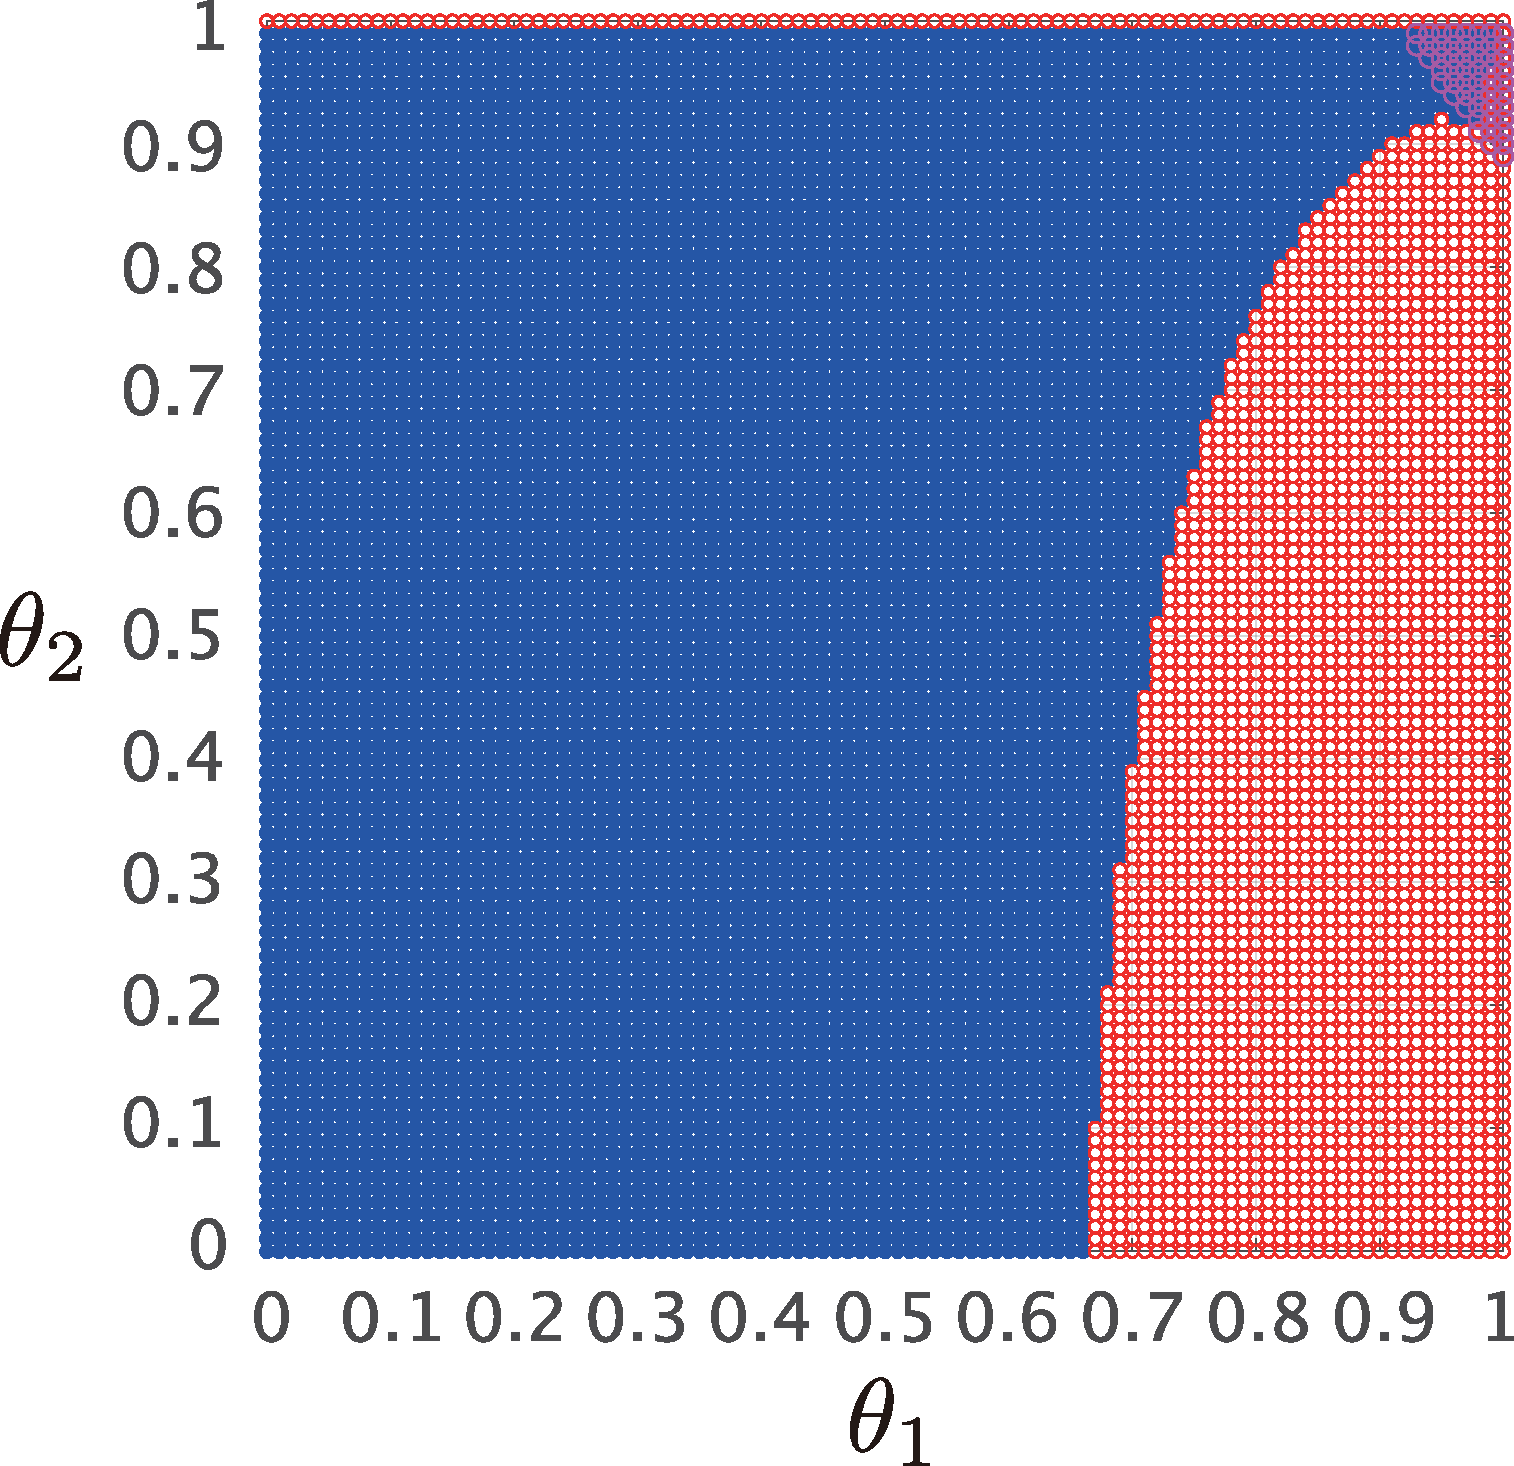
\includegraphics[width = .85\linewidth]{figs/gam01thm}
    \subcaption{ $\gamma=0.1$ }
  \end{minipage}
  \begin{minipage}{0.32\linewidth}
    \centering
    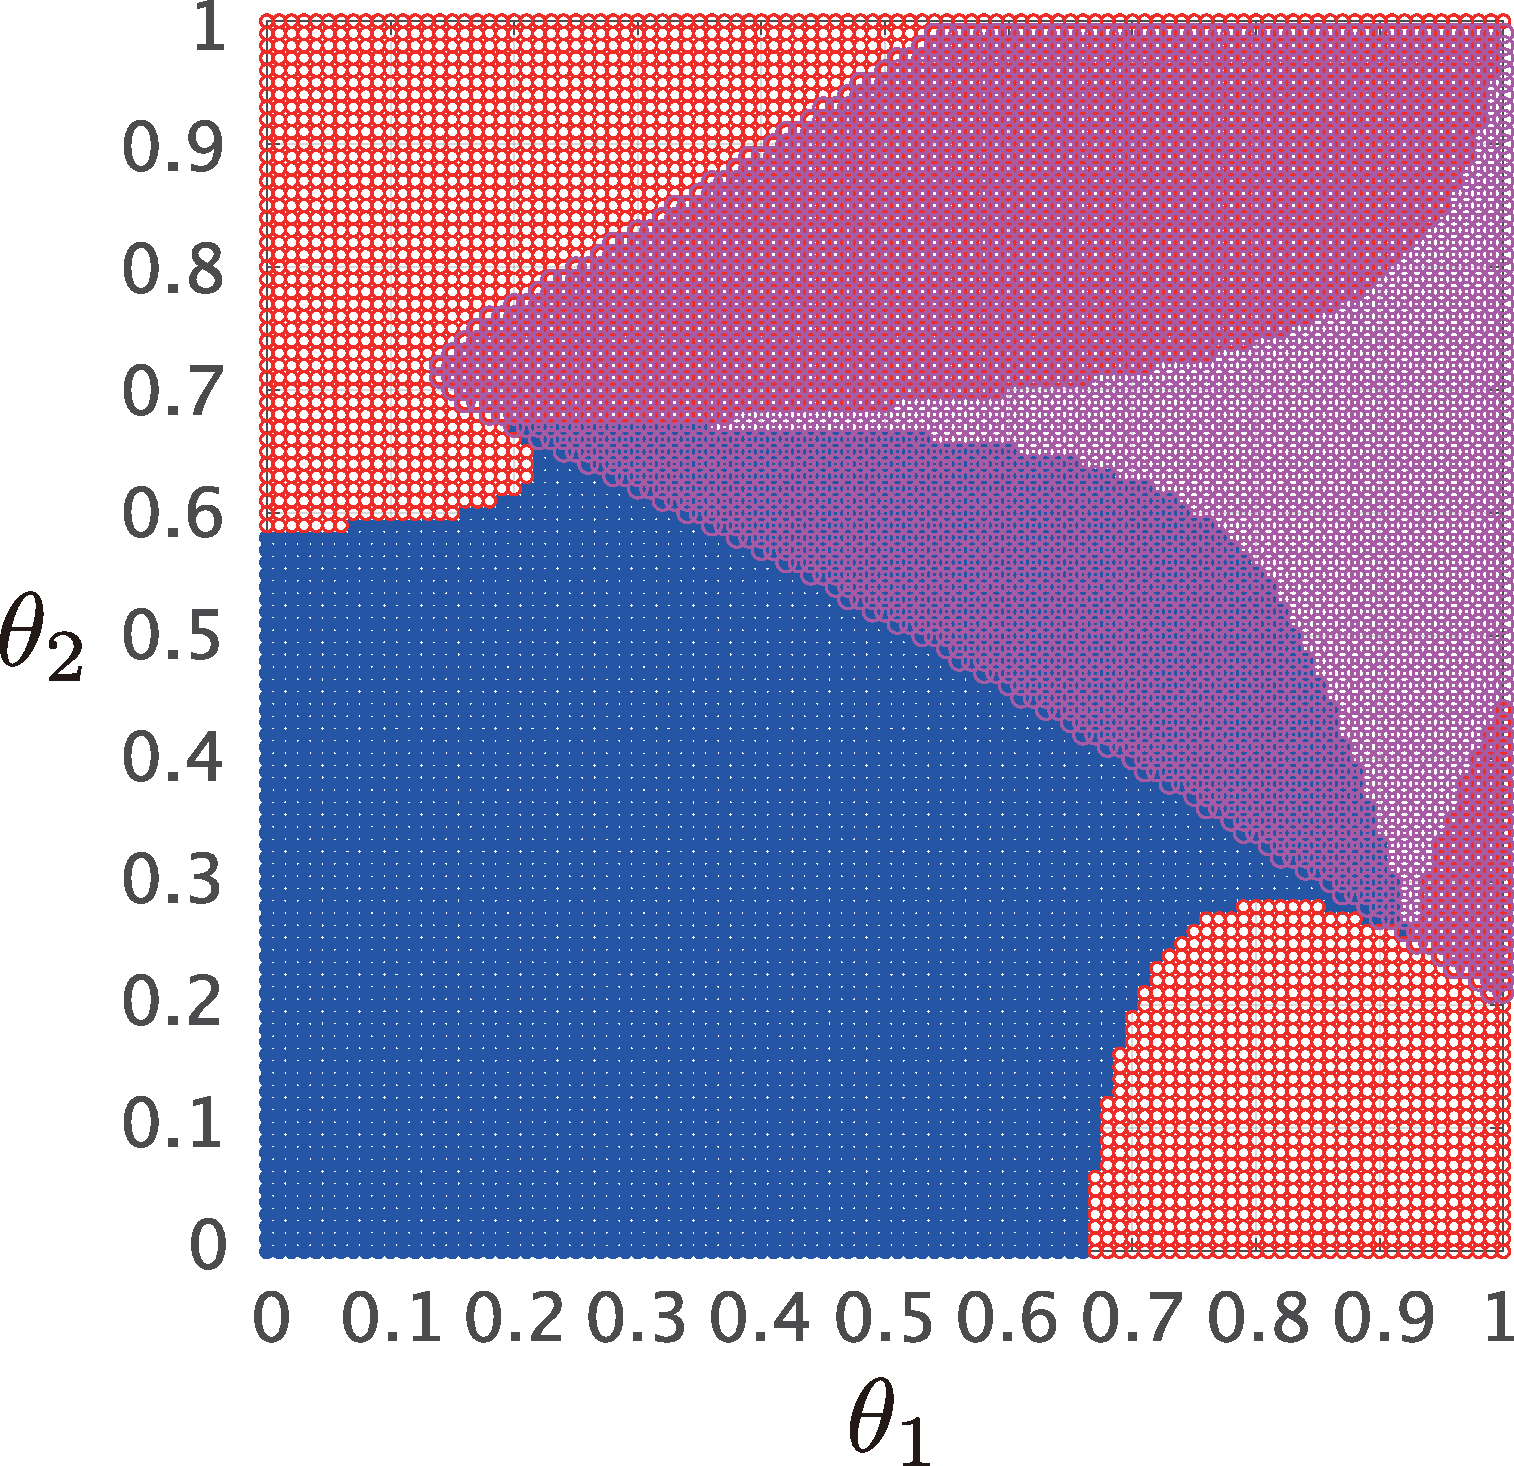
\includegraphics[width = .85\linewidth]{figs/gam2thm}
    \subcaption{ $\gamma=2$ }
  \end{minipage}
  \begin{minipage}{0.32\linewidth}
    \centering
    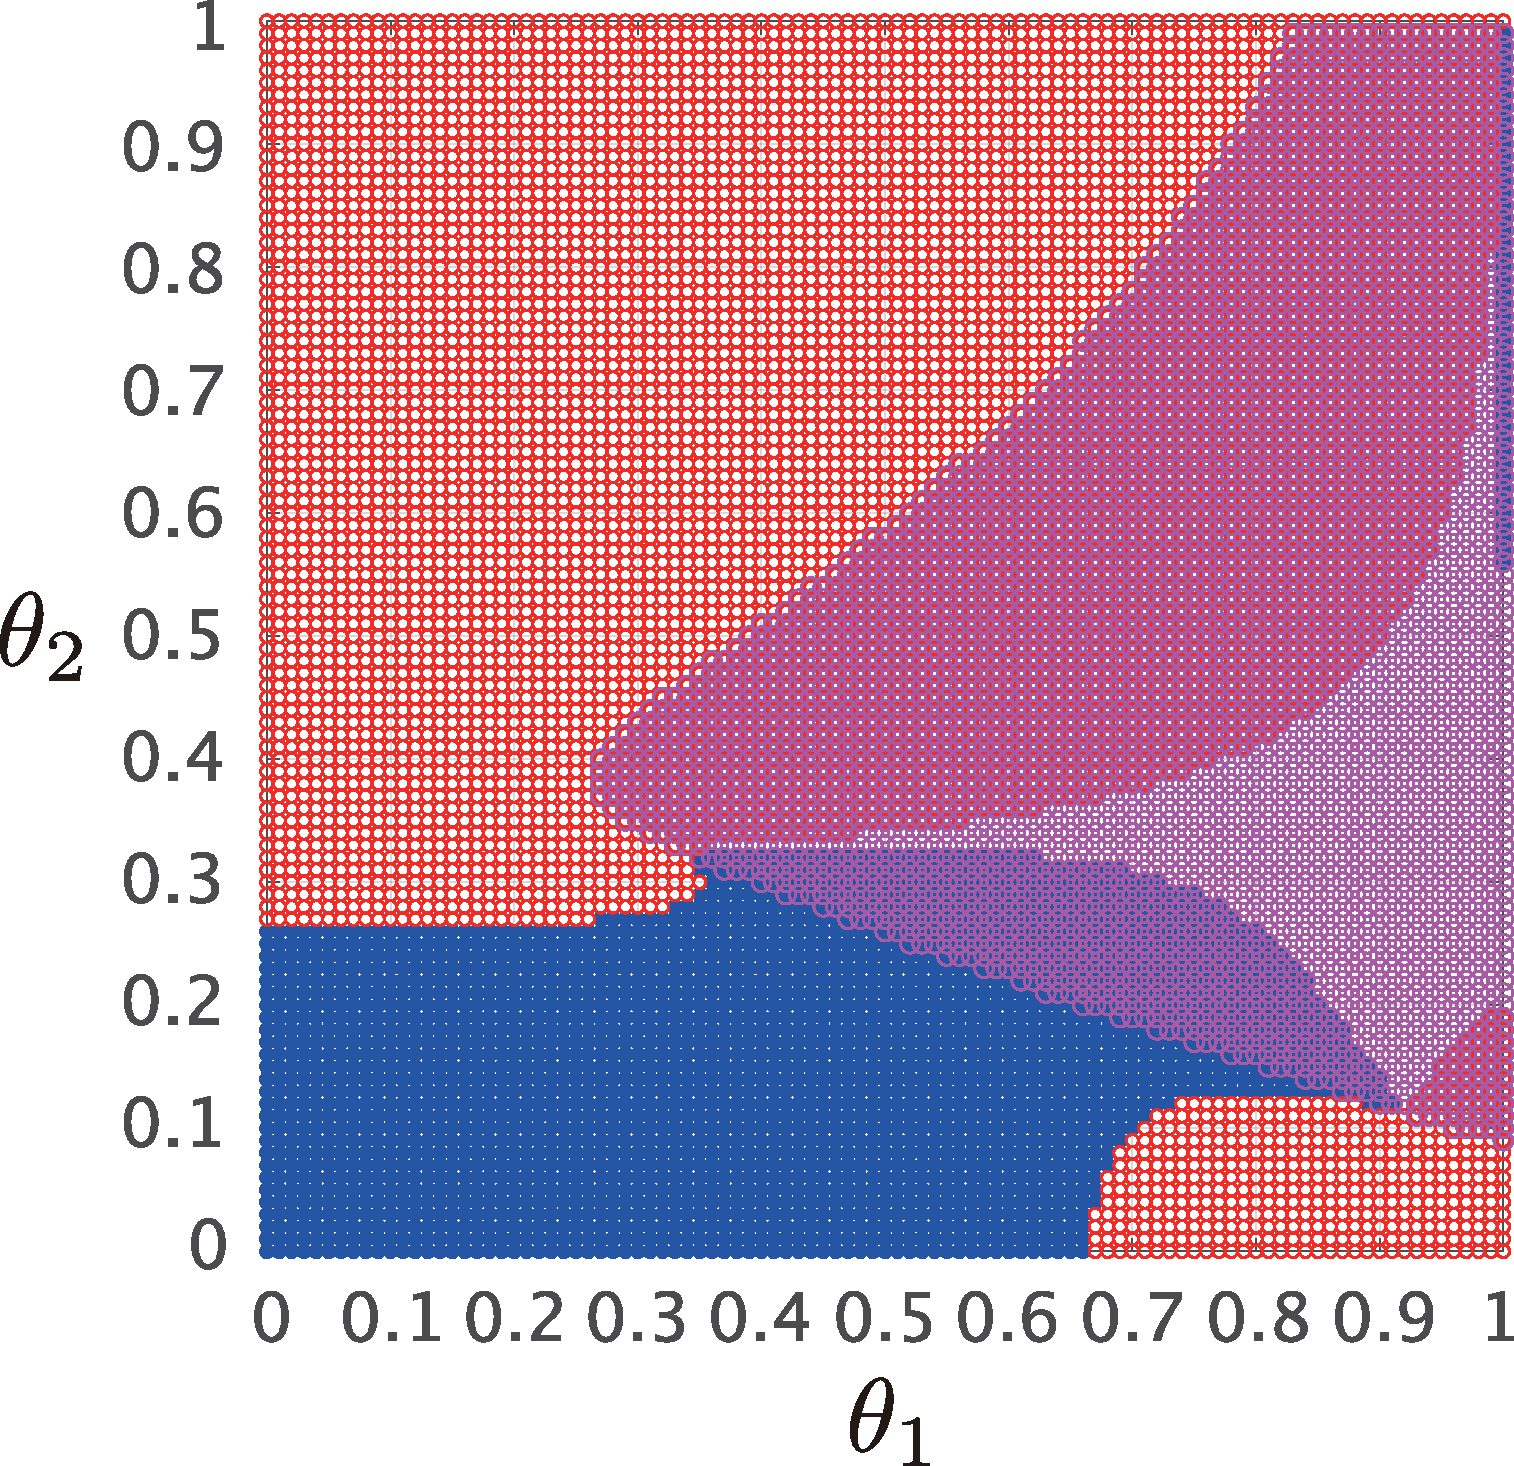
\includegraphics[width = .85\linewidth]{figs/gam5thm}
    \subcaption{ $\gamma=5$ }
  \end{minipage}
  \caption{例\ref{ex:linsyssim}の定数に対する定態安定性}
  \label{fig:gamthm}
  }
\end{figure}

\begin{figure}[t]
  \centering
  {
  \begin{minipage}{0.32\linewidth}
    \centering
    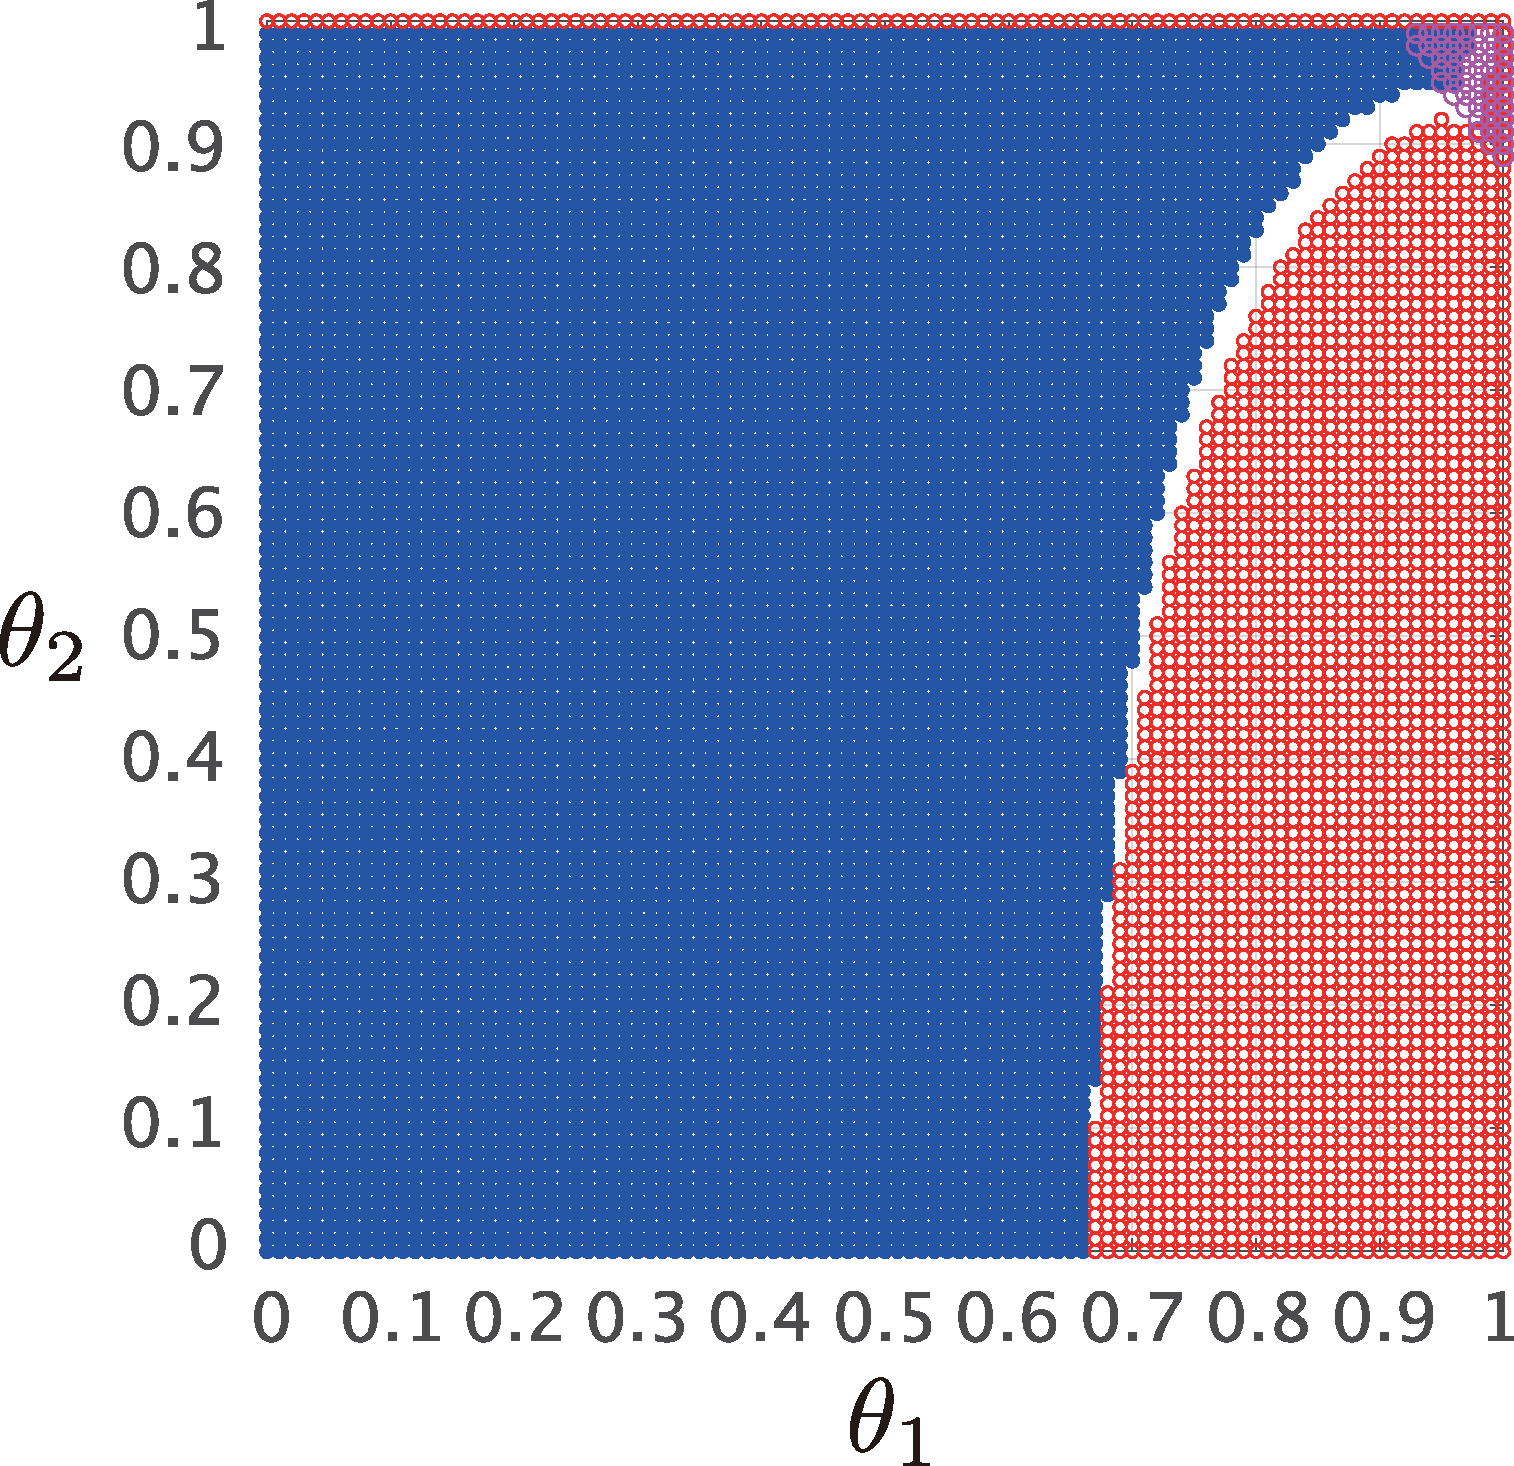
\includegraphics[width = .85\linewidth]{figs/gam01ex}
    \subcaption{ $\gamma=0.1$ }
  \end{minipage}
  \begin{minipage}{0.32\linewidth}
    \centering
    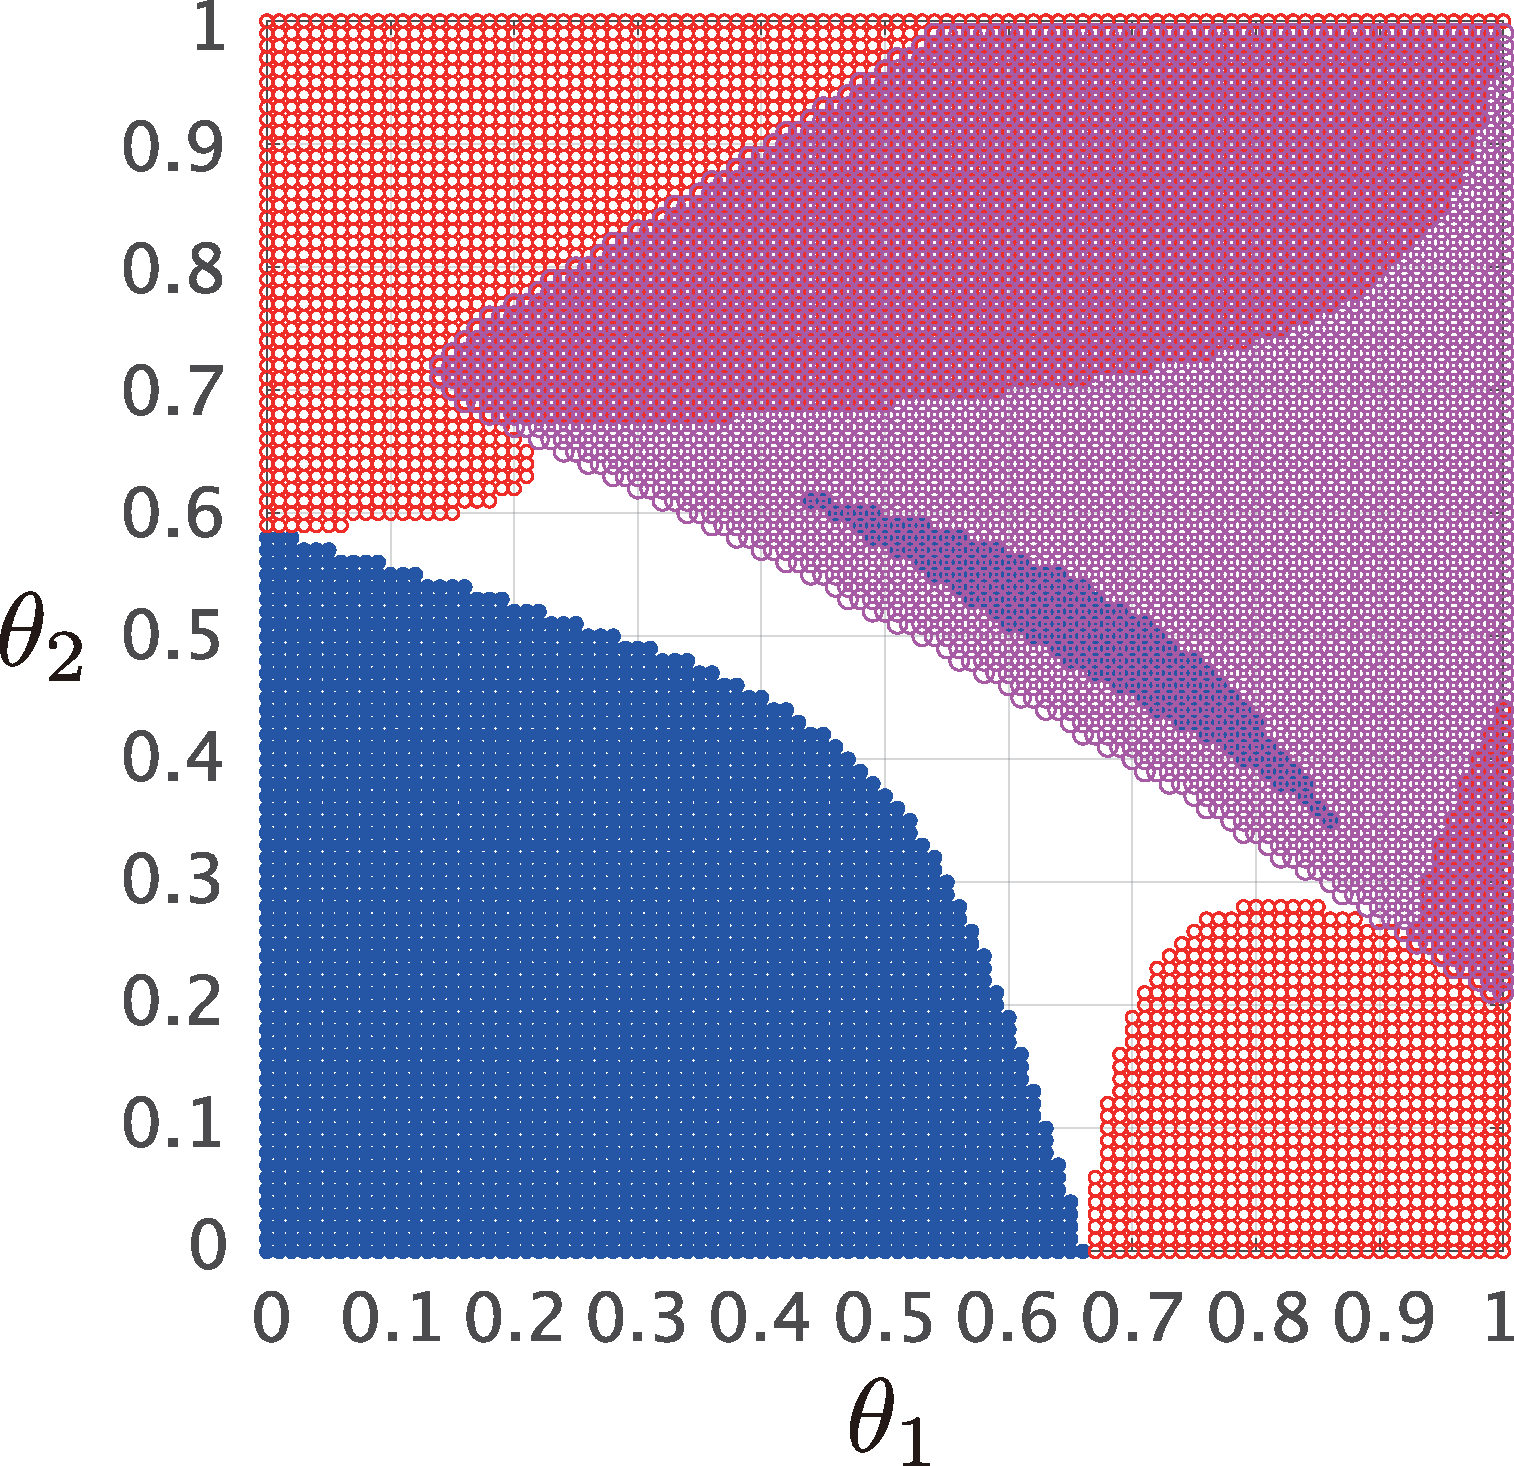
\includegraphics[width = .85\linewidth]{figs/gam2ex}
    \subcaption{ $\gamma=2$ }
  \end{minipage}
  \begin{minipage}{0.32\linewidth}
    \centering
    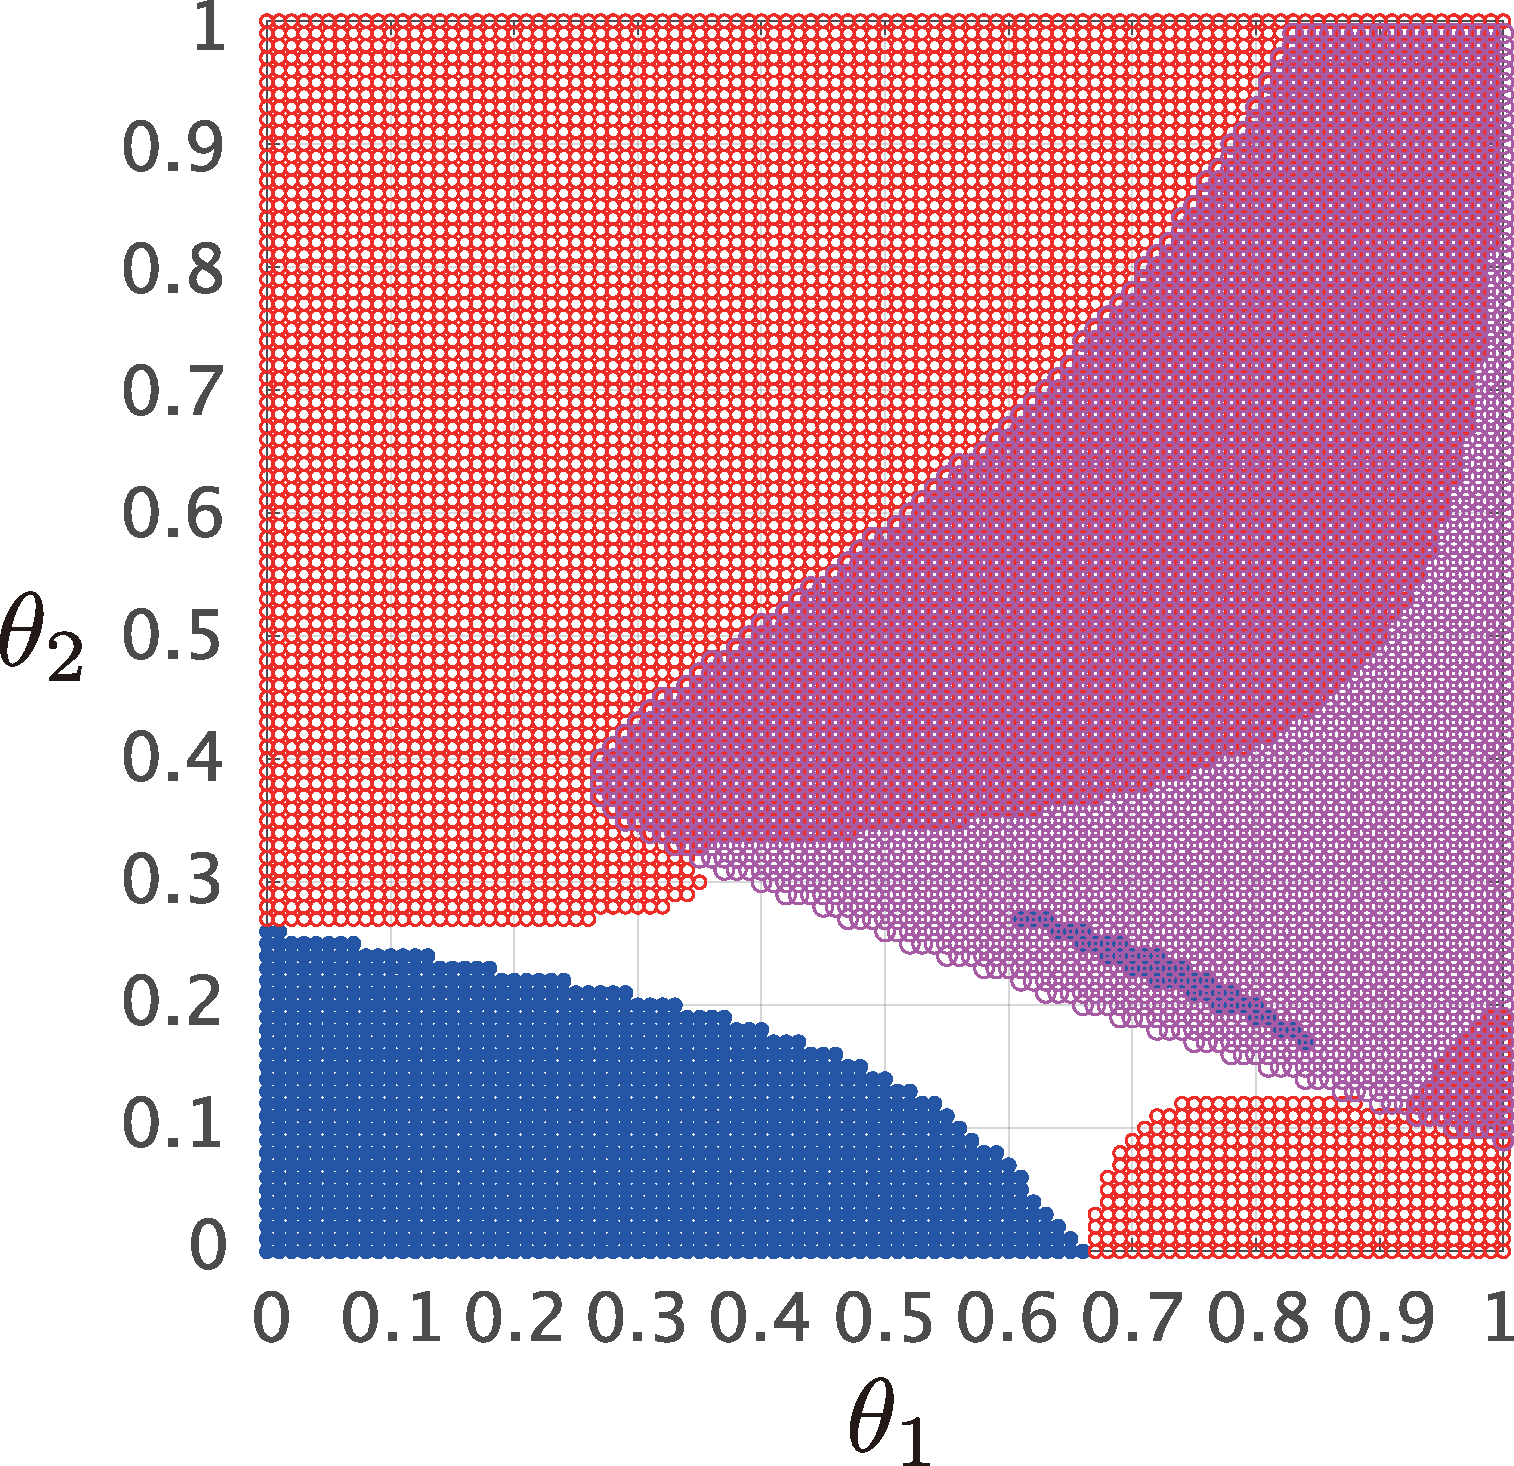
\includegraphics[width = .85\linewidth]{figs/gam5ex}
    \subcaption{ $\gamma=5$ }
  \end{minipage}
  \caption{定数の設定を変更した場合の定態安定性}
  \label{fig:gamex}
  }
\end{figure}


\begin{例}[受動送電条件に基づく定態安定性解析]\label{ex:linthm}
定理\ref{thm:sync}を用いて,例\ref{ex:linsyssim}で扱った3つの発電機から構成される近似線形モデルの定態安定性を解析してみよう。
発電機の物理定数などの設定は,すべて例\ref{ex:linsyssim}と同じであるとする。
受動送電条件(i)はすべてのパラメータに対して満たされていたため,
\ref{fig:gamsta}(a)--(c)には,受動送電条件(iii)$'$が満たされないパラメータの領域を重ねてプロットしている。
ただし,式\ref{eq:defL0}の$L_0$の固有値に実部が負であるものが含まれる場合を赤で示し,複素数の固有値が含まれる場合を紫で示している。
なお,$\theta_2=0$となる横軸上の領域が,受動送電条件(ii)が成り立つ場合を表している。

定理\ref{thm:sync}では,この赤や紫で示された領域が「ある物理定数の設定において近似線形モデルが必ず不安定となってしまう危険なパラメータ領域であること」が示されている。
また,受動送電条件(ii)が成り立つとき,すなわち,$\theta_2=0$である横軸上のパラメータに対しては,赤ではない値に$\theta_1$を設定する限り,それらの定数の値に依らず必ず近似線形モデルが定態安定性となることも示されている。

この結果で注目すべき点はつぎの2つである。
\begin{itemize}
\item 赤で示されているパラメータ領域は,上記の物理定数の設定で定態安定となる青いパラメータ領域の境界の一部を正確に捉えている。
\item 紫で示されているパラメータ領域は,定態安定となる青いパラメータ領域と重なる部分が存在している。
\end{itemize}
まず,1点目に関して,定理\ref{thm:sync}で示される受動送電条件(iii)$'$の必要性は,近似線形モデルが不安定となる発電機の物理定数の設定が少なくとも1つは存在することを意味している。
したがって,例\ref{ex:linsyssim}で設定されている特定の定数に対しては,定態安定となるパラメータ領域を必ずしも正確に捉えられるとは限らない。
一方で,実際に青い領域の境界の一部を正確に捉えられているという事実は,$L_0$が実部が負の固有値をもつ場合には,多くの場合で近似線形モデルが不安定となることを示唆している。

つぎに,2点目に関して,青の領域と紫の領域が重なっていることは,例\ref{ex:linsyssim}の物理定数の設定では定態安定である一方で,近似線形モデルが不安定化する定数が必ず存在することを意味している。
すなわち,青と紫が重なる領域は,発電機の物理定数などの値に依存して,定態安定である場合と定態安定でない場合が混在するパラメータ領域である。


参考として,定数の設定の一部を変更し
\begin{align*}
E_1^{\star}=2
,\quad
E_2^{\star}=4
,\quad
E_3^{\star}=6
,\quad
D_1 = 2
,\quad
D_2 = 1.5
,\quad
D_3 = 1
\end{align*}
とした場合の結果を\ref{fig:gamex}に示す。
基本的な傾向は,\ref{fig:gamsta}と同様である。
この図において現れている「白い領域」は,上記の物理定数の設定では近似線形モデルが不安定である一方で,不安定となる定数が必ず存在することまでは数学的に証明されていないパラメータ領域である。
具体的には,$L_0$は非負の実数固有値しかもたなかったが,近似線形モデルが何らかの理由で不安定であったパラメータ領域である。
このように,赤と紫の領域外のパラメータであっても不安定化の危険がないとは結論できないことに注意されたい。
この理由は,受動送電条件(ii)が成り立たない場合には,定理\ref{thm:sync}は定態安定性の必要条件のみを示しているためである。
\end{例}




%\bibliographystyle{myjunsrt}		% bib style
%\bibliography{reference}	% your bib database


\newpage
\end{document}






















